\documentclass[letterpaper,english, 12pt]{scrreprt}
\usepackage[T1]{fontenc}
\usepackage{array}
\usepackage{graphicx}
\usepackage{float}
\usepackage{titlepic}
\usepackage{multirow}
\usepackage{longtable}
\usepackage[bookmarks=true]{hyperref}

\newcolumntype{C}[1]{>{\centering\let\newline\\\arraybackslash\hspace{0pt}}m{#1}}

\title{Musical Heart Rate Adjuster}
\author{Group \#12 \\ https://github.com/revan/HeartRateAdjuster \\ 
\\Kenny Bambridge, Jonathan Chang, Samani Gikandi,
\\Tae-Min Kim, Nikhil Shenoy, Revan Sopher}

%\textsc{Software Engineering 14:332:452}


\begin{document}
\titlepic{
\includegraphics{img/title.png}}
\maketitle

\tableofcontents

\section*{Team Profile}
\begin{description}
	\item[Nikhil Shenoy] C++, Python
	\item[Revan Sopher] Android programming, web programming, Java, Python
	\item[Tae-Min Kim] Java, C++, Python
	\item[Samani Gikandi] Java, C, Ruby, Network programming, Device driver/firmware programming
	\item[Kenny Bambridge] IOS programming, web programming, Java, Python
	\item[Jonathan Chang] documentation, organization, C++
\end{description}
 
\chapter{Customer Statement of Requirements/Project Proposal}
 
\section{Problem}
There seems to be a growing concern over the bevy of health-related issues that society faces: cancer, obesity, heart diseases. This is evidenced by the estimated \$25.9 billion that consumers spent on fitness membership in 2013 or the government's seemingly carte blanche spending on "perfecting" the healthcare.gov website. While it is impossible to completely eliminate health problems, we focus on a small, albeit interesting subset of the health industry - personal health monitoring. Just like "an apple a day keeps the doctor away," our project seeks to maintain the personal health of an individual, keeping him in the best physical shape possible, and reducing the risk of health problems. \\
 
\subsection{More Specifically}
Lack of education about proper fitness is a widespread problem. Many people in the country would like to exercise and stay in shape, but only a small subset of those people know how to monitor their health in a way that allows them to stay fit. There are several methods out there which people can use to get the proper information; tools such as fitness blogs, the President's Council on Fitness, Sports, and Nutrition, and the classic visit to the doctor's office are all excellent examples. However, many people don't know about those methods or choose not to utilize them, and they do their body a disservice by performing exercises that could be detrimental to their health. The Internet is littered with articles such as "9 Exercises You're Doing Wrong" and "The 7 Fitness Myths You Need to Know". With information like this readily available to exercisers, it can be hard to find correct information. And even if one does find correct information, he must check to see if that information applies to a person with his body shape and size. The general problem of finding correct exercise information is that there is no set standard; there is no "one size fits all" set of guidelines which one can follow to have an effective workout. Everybody's body responds differently to different exercises, so the best that the medical community can do is to provide a set of recommendations for people of the most average body type. While this set of recommendations is good in the general, they will never tailor to the needs of one's body and workout. Finding the correct exercise information for one's body type is quite a difficult problem, and it will continue to be a problem until a solution is provided to track each person's exercise routine.\\
 
Of all the different metrics for measuring the quality of one's fitness, heart rate is the most important factor in determining whether a workout was effective. Monitoring one's heart rate is useful because it determines whether the exerciser is performing his exercise safely as well as successfully. Experts recommend that one's target heart rate during exercise should be between 60-85\% percent of the maximum heart rate, and that anything higher than 85\% increases cardiovascular and orthopedic risk to the exerciser. Naturally, the target heart rate varies for people of different ages, so one should always take this into account before starting a fitness regimen. Also, the frequency of exercise before the new regimen should be considered. If one has not exercised frequently before starting the new regimen, then he should start exercising at a rate that is towards the lower end of the target heart rate zone and then gradually increase his activity once his body gets accustomed to the exercise. Heart rate is a significant, if not the most important, factor in determining whether a workout was done correctly and effectively, and it must be monitored closely in order to prevent injury.\\
 
Unfortunately, there are people who don't know how to correctly monitor their heart rate, and they mistakenly create a certain fitness plan based on wrong information and end up not optimizing their workout. They go to the gym, run on the treadmill at a light pace, and consider that enough to maintain their health. They do not check their heart rate and make sure they are in the safe region of activity. This critical lack of measurement affects the entire workout. For an exercise to be effective, one must maintain a heart rate that is within the target range for an extended period of time. If not, the exerciser either puts himself at risk of injury or completes a workout that does very little to improve his fitness. Some use exhaustion and soreness after a workout as a judge of an effective workout. Although these methods do give an indication as to how effective the exercise was, they do not provide an insightful and accurate description of one's health. As a result, these people continue bad habits and routines that hinder their progress to stay fit; in fact, they may not be even making progress.\\
 
A solution to the problem of uninformed exercise must have three main components; it must include all relevant medical data such as heart rate information, create a fitness plan that fits relatively well to the client's body, and provide the client with feedback about the effectiveness of his workout. Once all these components come together, the client will be able to correctly monitor his health during exercise and get the most out of his workout.\\
 
\subsection{Background}
A healthy lifestyle depends upon a plethora of factors including environment, nutrition, socialization, and mental stability. However, we identified physical fitness and sleep as the two key factors to leading a healthy lifestyle. Their importance cannot be overstated.\\
 
Physical fitness or exercise fortifies the body, allowing one to stay in shape, avoid injuries, develop confidence, become stronger, and sleep better. Sufficient physical activity can reduce the risk of such symptoms as stress, depression, diabetes, high blood pressure, osteoporosis, and obesity.\\
 
Meanwhile, sleep is critical to the mind. It refreshes the brain, helps with daily functioning, uplifts one's mood and emotional well being, increases productivity, and improves learning and memory. "Good" sleep can lower the probability of contracting the following: heart disease, kidney disease, high blood pressure, diabetes, and stroke.\\
 
\subsection{Devices and Specifications}

Heart Rate monitor: \\
Uses Bluetooth or ANT+ to connect to smartphone \\

Smartphone: \\
Needs to be running Android 4.3+ \\
Needs to have radio supporting Bluetooth 4.0+  \\
\\

\section{Solution}
It has been well documented that exercise and sleep both hold a significant impact on heart rate[14-15]. However from experience, we believe that the link between exercise and sleep and heart rate holds true for the converse as well. One of the targets of a good workout is an increased heart rate. On the other hand, high-quality sleep entails a decreasing heart rate.\\
			 
Our proposed solution is designed to affect people's health by providing limited control to their heart rates. Our Musical Heart Rate Adjuster is targeted to operate in two areas where it can be the most effective - workouts and sleep - which in turn offer the aforementioned health benefits. We do not plan on adjusting heart rate with the intent of skipping the rigors of exercise or the process of falling asleep; on the contrary, we wish to adjust heart rate to induce better quality workouts and sleep.\\
			 
Our plan is composed of a few steps. First, we intend to increase the effectiveness of workouts by matching heart rate to an appropriate selection and tempo of music. This music can be adjusted accordingly to stimulate heart rates to reach a desired intensity of exercise. The music, which will be discussed later, performs the task of simulating workout difficulty. As an added benefit, studies have shown exercising while listening to music to provide many benefits, such as increased motivation and endurance, distraction from otherwise unbearable stress, and increased heart rate, among others.\\
			 
Then, we seek to improve the quality of sleep by finding soothing music to gradually slow down a user's heart rate. In this instance, we use music as an instrument to aid users in falling asleep more quickly, and hopefully improve the performance of their rest. Listening to right music can also improve the quality of sleep; for instance, music by classical composer Mozart has been shown to increase health factors such as relaxation and mental stimulation.\\
			 
\subsection{Music}
We utilize music to affect heart rate in two ways. In addition to identifying and playing music with speeds in the same vicinity as heartbeat, we also wish to be able to adjust the tempo of the music. A simple compound microscope has both a coarse adjustment knob as well as a fine adjustment knob. Our song library will organize songs into different categories, acting as a coarse adjuster for heart rates. Meanwhile, to add a little fine-tuning to adjust the heart rates, we will either write or find an existing application for an audio tempo changer. Given current heart rate, and subsequently, current music tempo, we will continually adjust the music tempo while measuring for changes in heart rate. This will occur until we hit the specified target heart rate, give or a take a few BPM. Thus, if there is no difference in heart rate, either the targeted heart rate has been reached - otherwise,  the music tempo has not been adjusted enough.\\
			 
We are interested in analyzing the magnitude of the effect of our music application on heart rate and finding a rough correlation based on the data that the MOTOACTV provides. All parties should remember, however, that correlation is not causation. While we take the assumption that the general public will react to music in similar ways (music with a slower tempo will decrease heart rate while music with a higher tempo will increase heart rate), it is difficult to know how every individual will react to the same music and can never be 100 percent accurate.\\

This will probably take some experimentation with test subjects in several situations such as rest, running, weight-lifting, and playing basketball. Time-permitting, we will also find the ability of music to slow down heart rate and affect sleep by analyzing sleep monitor graphs. As a side experiment, we could measure the effect of several well-known classical songs on sleep quality.\\
			 
Finally, we will be able to develop an algorithm for ranking the songs that induce the best performance. Even better, we could potentially toy around with machine learning to have our algorithm improve after more and more data sets. With the application of machine learning, each user's individual MOTOACTV device may correct itself in the case that a specific user does not follow the general trend as stated previously (a user's heart rate might increase from slow music rather than fast music). This way, our MOTOACTV will be able to increase both exercise and sleep performance through our own custom music player application, located on and loaded by the device. This application will utilize the user's music library stored locally on the device's memory.\\

\subsection{Database}
Users will want to monitor their personal health status, so our project will allow the user to view his workout data directly on his phone. This eliminates the inconvenience of having the user log in to a personal account on a website to view his data, because everything he needs will be on the phone itself. All the data collected from the workout will be stored locally on the phone, and the system will perform the necessary database calls to retrieve that data. That data will be processed and formatted into different graphs that will display the correlation between music and heart rate.\\


\subsection{System Architecture Diagram}
This diagram highlights our system architecture: Our heart rate monitor senses the
user's BPM and transmits the data to the Android phone via Bluetooth as requested
by the app. The phone then uploads the data to the server and database
which processes the data. The system is then able to select the appropriate
songs, and then display suitable graphs once the workout is completed.\\

\begin{center}
	\begin{figure}[H]
		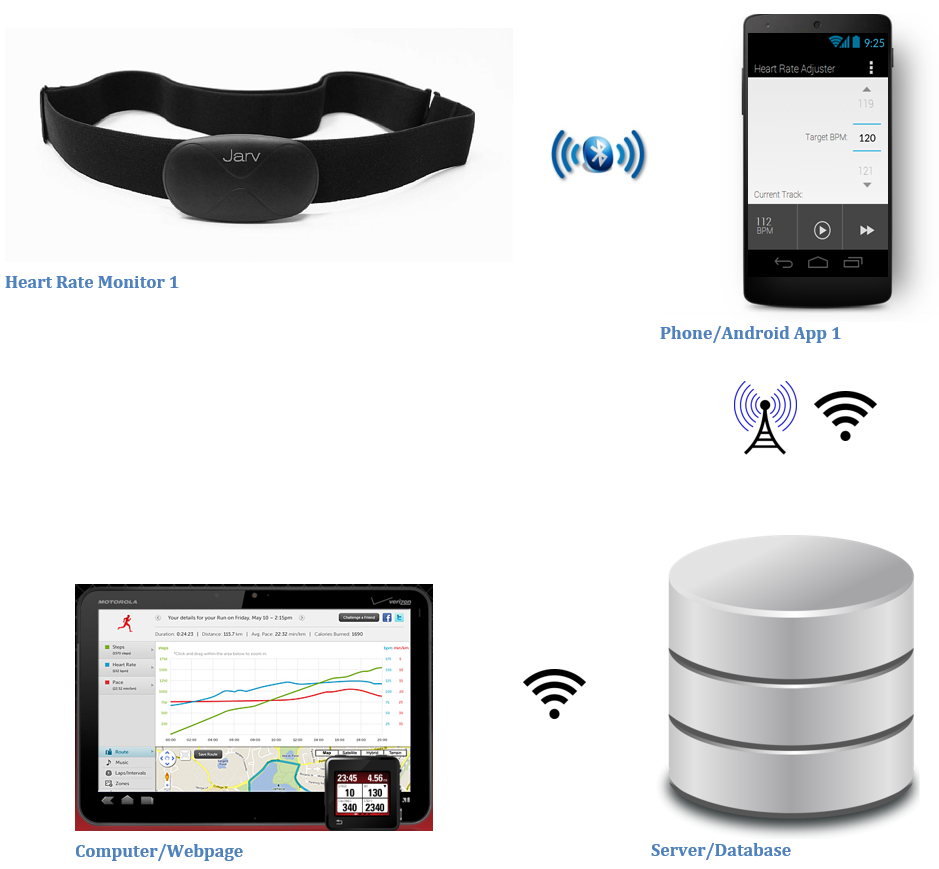
\includegraphics{img/system_architecture.png}\\
		\caption{System design}
	\end{figure}
\end{center}

\subsection{Product Usage}
\begin{itemize}
	\item The heart rate monitor should only be worn while it is in use - only while the user is exercising. While it is safe to wear the heart rate monitor during other times, there will be no benefit unless the application is currently running. 
	\item Users may choose to use the Musical Heart Rate Adjuster while not sleeping or exercising if they wish to adjust their heart rate for alternate reasons (possibly for playing video games or preparing for an exam). 
	\item The user will run the android application, and then input a target heart rate. The software will then choose a song based on your current heart rate and begin to either raise or lower it. Once the target heart rate is obtained within a certain tolerance, the software will work to maintain this heart rate rather than increasing/decreasing it.
	\item Music will be selected from the user's own personal music library (which should be stored on the flash memory of the Android device) to either increase or decrease the user's heart-rate. Music will be played by our software.
	\item The software will select and play music according to the user's current heart rate in real-time as it receives information from the connected heart rate monitor.
	\item Music will be delivered through the headphone jack on the Android device or through any bluetooth device.
	\item Receive information on the songs that are listened to in relation to their usage of the Android device. (What songs were listened to, which songs were the most effective at changing their heart rate, etc.)
\end{itemize}

\subsection{Product Ownership (tentative)}
Our team will be divided into three smaller sub-teams of two individuals each, the pairings listed below. Each sub-team will be responsible for music, hardware, or web and provide a brief description of their work on a shared Google drive folder. They will also include the necessary UML diagrams and charts. Every week (or bi-week) we will meet together for 1-3 hours during the timeframe determined by When2meet. During the meeting, we will have a specific agenda that primarily involves the week's progress and upcoming deliverable. Our discussion will probably be centered along the following questions: 1) What did you work on this past week? 2) What do you plan on working on next week? 3) Are there any changes that need to be made to the project? Every week, a different team member will take the lead for the next deliverable to ensure that everything is on time.\\

\begin{itemize}
	\item Kenny and Samani will develop a system to select or modify a track based on requested BPM. If possible they will incorporate machine learning into the system.
	\item Jonathan and Nikhil will work on a database that receives, stores, and processes the data from the Android device. They will also be responsible for creating the graphs that measure different metrics of the workout.
	\item Revan and Tae-min will program the Android application and work on interfacing with the heart rate monitor.
\end{itemize}

\section{Glossary of Terms}
\begin{description}
	\item[Electrocardiography (ECG)] ECG is an interpretation of the electrical activity of the heart over a period of time as measured across the thorax or chest. This interpretation is produced by attaching electrodes to the surface of the skin. This is generally used to measure the heart's electrical conduction system by picking up electrical impulses generated by the polarization and depolarization of cardiac tissue.

	\item[Beats per Minute (BPM)] BPM is the amount of times that the heart beats given one minute of time.

	\item[Resting Heart Rate] The resting heart rate is the heart rate measured while the subject is both awake and inactive, not having performed physical activity prior. This resting heart rate, measured in bpm, is the initial value that the user should have before using our device to raise or lower their heart rate.

	\item[Database] Databases are a place to store information. In our case, this is where we will store and process important data received from our health devices, allowing our system to simply act as a pleasant interface for the user.

	\item[Target Heart Rate] The target heart rate is the heart rate which the user wishes to achieve. This will be lower than the recorded resting heart rate if the user is attempting to sleep, and higher than the recorded resting heart rate if the user is planning to work out. The user's maximum heart rate is based on how old the user is (220 minus the user's age), and the recommended target heart rate while exercising is between 50 and 85 percent, depending on how active the user normally is. While sleeping, people's heart rates generally drop approximately 8 percent from their resting heart rate, so the user's target heart rate should be approximately [(heart rate before sleeping)*0.92]

	\item[Smartphone] Smartphones are mobile phones which contain features that are more advanced than basic mobile phones. In our case, any Android device which has the capability to use Bluetooth will suffice to interact with the sensors which will be put on the body.

	\item[Heart Rate Monitor] A device which is able to monitor the user's heart rate. In our experiment we will be using a third party heart rate monitor (worn as a chest strap) which has sensors that are connected to the skin along with the MOTOACTV watch. The chest strap will record the heart rate while the watch will display the user's current heart rate in real time.
\end{description}

\chapter{System Requirements}
Based upon our consumer needs, we derived a list of requirements for our system to
possess. For features that must be implemented by the system, we state that "The
user shall," whereas for features that are preferred, but not "mandatory," we state
that "The user should." For each requirement, we assign an identifier in the form of
REQ-x, as well as a priority weight from 1 to 5. A higher priority weight indicates
that the corresponding requirement is more essential to the success of the project,
and more critical to fulfilling the customer's needs.\\

\section{Functional Requirements}
\begin{center}
	\begin{tabular}{|C{2cm}|C{2cm}|C{8cm}|}
		\hline
			Identifier & Priority & Description\\
		\hline
			REQ-1 & 5 & The system shall log user BPM data using the Heart Rate Monitor sensor during active periods.\\
		\hline
			REQ-2 & 4 & The system shall allow user to select a target heart rate on the Android application.\\
		\hline
			REQ-3 & 3 & The system shall determine a song to play based on whether the target heart rate is greater than or less than the resting heart rate. \\
		\hline
			REQ-4 & 5 & The system shall play the designated song through either headphones or Bluetooth speakers to adjust user heart rate. \\
		\hline
			REQ-5 & 3 & The system shall store the BPM data of each song in the database. \\
		\hline
			REQ-6 & 2 & The system shall at the very least, output graphs relating BPM versus song speed.\\
        \hline
    \end{tabular}
\end{center}
\begin{center}
	\begin{tabular}{|C{2cm}|C{2cm}|C{8cm}|}
		\hline
			REQ-7 & 1 & The system should adjust the tempo of the song to attempt to match the user's BPM and stop when within a defined range. \\
		\hline
			REQ-8 & 1 & The system should allow the user some control when they use the "Display Statistics" feature. That is, they should be able to customize the details of how the data is displayed (type of graph or specific categories of data).\\
		\hline
			REQ-9 & 1 & The system should rank the songs that induce the best performance and use machine learning to improve the song selection algorithm. \\
		\hline
                        REQ-10 & 1 & The user should be able to change the current song if he is unsatisfied with it. \\
                \hline
                        REQ-11 & 1 & The user should be able to view his current heart rate as long as the chest strap is recording that information. \\
		\hline
			REQ-12 & 1 & The user should be able to pause the current track if he needs to interrupt his activity for some reason \\
		\hline
	\end{tabular}
\end{center}

Our functional requirements spell out the behavior of our system and reaction to
user input. Our system is composed of several aspects such as the heart rate
monitor, android device, server and database. These requirements
describe some of the interactions between these components and the effects that
the system as a whole produces. The images in the appearance requirements section
later on provide more insight on the requirements and functionality of our system. \\

For our system to be able to accomplish any of its goals, it must first be able to record the relevant BPM data. Therefore, our REQ-1 is of utmost important. There is, however, an important scenario we must consider. If the the heart rate sensor is removed (accidentally or intentionally) while the user is active, any later data collected and song played may be skewed. Thus, the time in between active periods is irrelevant and will have no effect on the software.\\

In regards to music playback, it is desirable for our system to do the data processing and song section, to reduce the burden on the user. Again, after collecting the BPM data and storing it in our database, our system will use a pre-determined algorithm to analyze song tempo and bpm correlation to determine song selection (REQ-3 \& REQ-5). As for physical playback, the choice of whether to use headphones or speakers will not have any effect on the performance of the system. The choice is simply the user's preference (REQ-4).\\

To safeguard against mistakes, and prevent negative side-effects, if the system makes an incorrect decision, there will be no negative consequences on the user's health. It should be able to re-adjust once it realizes that the song's tempo does not match the user's current and target heart rates (REQ-7). For REQ-9, this ranking system will be completely local and only relevant to the user of the system. This is just an optional improvement to our system to enhance the user's experience.\\


\section{Non-Functional Requirements}
\begin{center}
	\begin{tabular}{|C{2cm}|C{2cm}|C{8cm}|}
		\hline
			Requirement & Priority Weight & Description \\
		\hline
			REQ-13 & 5 & The Android interface shall have a minimal number of navigation menus; the user should not need more than three taps to find the information he needs \\
		\hline
			REQ-14 & 5 & The user shall not be able to directly modify any data in the database. All data must be programmatically gathered and processed \\
		\hline
			REQ-15 & 3 & The user should wear the device only when the user wishes to alter their heart-rate; the device will not provide useful information if it is worn when the user does not plan to increase or decrease their heart-rate. \\
		\hline
			REQ-16 & 3 & The Android application should be intuitive and simple to use. \\
		\hline
	\end{tabular}
\end{center}

Meanwhile, our non-functional requirements are more descriptive than practical,
listing the qualities of our system. These requirements are based on the term
FURPS+, which includes functionality, usability, reliability, and performance.

\section{On-Screen Appearance Requirements}

This section contains mockups of the Android application's user interface.
Although the arrangement and display is subject to change, these images contain all the essential information that needs to be conveyed to the user, as well as all the necessary inputs. \\
The inputs used while exercising, such as the BPM sliders and the music controls, take up a large amount of screen space to facilitate active use. Information display, such as the current track and BPM, is placed unobtrusively around the input methods. The configuration settings are hidden in a drop-down menu, as per the Android design standard.\\

\begin{figure}[H]
	\centering
	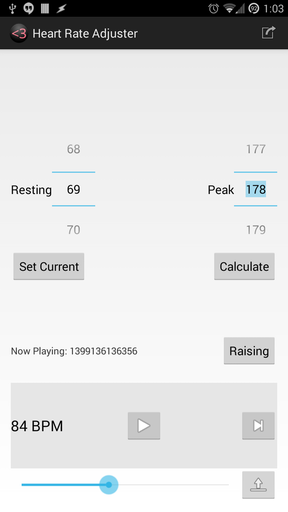
\includegraphics{img/mobile_ui/1.png}\\
	\caption{The main screen of the app provides a menu button, selectors for Target Peak and Resting BPM, a display of the current track, a display of the current BPM, and the option to Play/Pause and Skip the current track.}
\end{figure}

\begin{figure}[H]
	\centering
	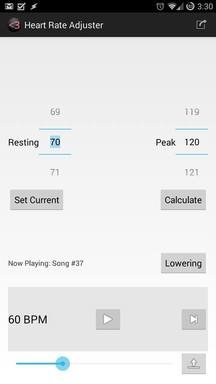
\includegraphics{img/mobile_ui/2.png}\\
	\caption{Pressing the ``Raise/Lower'' button toggles between attempting to raise or lower the BPM.}
\end{figure}

\begin{figure}[H]
	\centering
	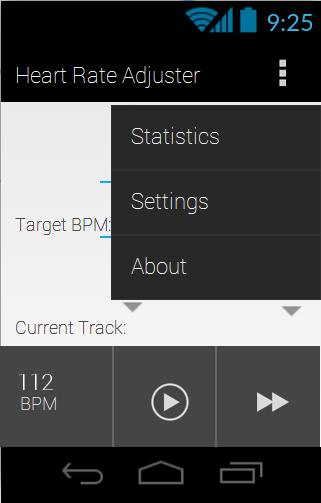
\includegraphics{img/mobile_ui/3.png}\\
	\caption{Pressing the menu button opens the context menu, providing the option to view statistics, edit settings, and view information about the app.}
\end{figure}

\begin{figure}[H]
	\centering
	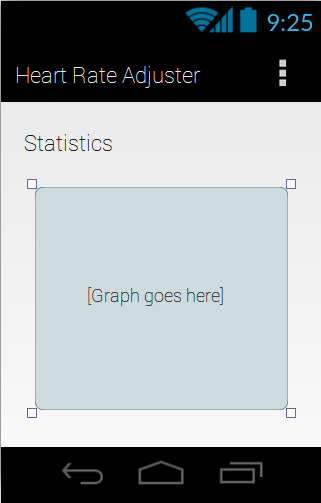
\includegraphics{img/mobile_ui/7.png}\\
	\caption{Selecting the Statistics option from the context menu displays a graph of user heart rate and song transitions.}
\end{figure}

\begin{figure}[H]
	\centering
	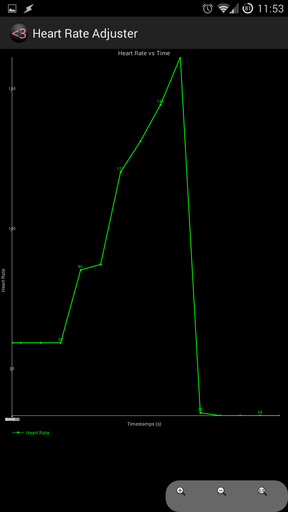
\includegraphics{img/mobile_ui/4.png}\\
	\caption{The settings page allows the user to open a menu to Log in, to edit the location of the media library (this is done via the OS's directory selection), and configure additional parameters such as music generation (if there is time to implement this feature).}
\end{figure}

\begin{figure}[H]
	\centering
	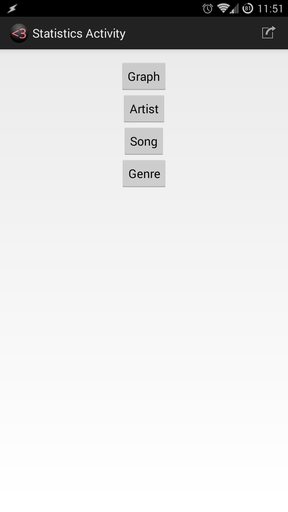
\includegraphics{img/mobile_ui/5.png}\\
	\caption{Selecting the Log in option prompts the user for their credentials.}
\end{figure}

\begin{figure}[H]
	\centering
	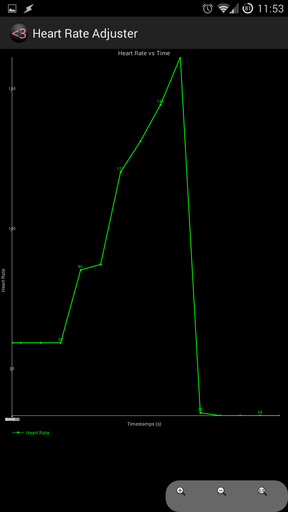
\includegraphics{img/mobile_ui/6.png}\\
	\caption{Selecting the About option from the context menu provides a description of the application.}
\end{figure}


\section{Organization}

\subsection{Stakeholders}
Stakeholders include individuals and organizations which are interested in the completion and use of a given product. The amount of stakeholders and different types of stakeholders relies on the versatility and ease-of-use of the product in question. Due to this software's very simple interface and design, stakeholders may include users of all ages and multiple types of organizations who are interested in obtaining easier sleep or a more energetic workout. Examples of potential stakeholders include:
\begin{enumerate}
	\item Individuals who are interested in maintaining their health personally without outside help. With the many functions of the application, users have the capability of maintaining their health without the need to consult other people. People who are introverts or do not have easy access to another person who is able to easily analyze the individual's personal health would be very interested in this application. After running this application through their workout or sleep, users can easily consult the graphs which are produced rather than consulting a personal trainer or doctor about their health.
	\item Organizations that specialize in helping people fall asleep. Rather than having to prescribe pills to every customer who has trouble sleeping, they will have the option to suggest this product to the customer for minor cases. While prescribing pills may tend to have slightly more dangerous side-effects, our product does not introduce any chemicals to the body which may potentially cause harm to the consumer. Organizations who are interested in a cleaner alternative to help people with their sleeping problems would be stakeholders for this product.
	\item Organizations that specialize in promoting exercise and personal health. Not only does this product help those who are trying to sleep, but also those who wish to be more fit. While personal trainers may know how to help the customers and be great motivators, organizations may be interested in helping a larger pool of customers without having to increase the amount of hands that they have working. With this product organizations may grant customers the option of being self-sufficient, helping to increase self-esteem, as well as a great motivator as the application works to increase the user's heart rate allowing them to push onward and burn calories easily.
	\item Organizations interested in monitoring and researching people's health. While there are many users who are able to use the product's graphs and understand how their health and workout are, there are many users who still prefer the assistance of outside sources. This product may also be used by these outside sources to help them collect extra data on an individual's health. Rather than having the customer come to their location and run a couple tests in a single day, the organization will have the ability to provide this product to the customer and collect more regular data to understand the customer's day-to-day life rather than a couple of tests run at their office.
\end{enumerate}

More specifically, this product may see stakeholders in:
\begin{itemize}
	\item Personal Trainers
	\item Athletes
	\item Coaches
	\item Doctors
	\item Researchers
	\item Pharmacies
	\item Therapists
	\item General population
\end{itemize}

\subsection{Actors and Goals}
Actors can be defined as are people or devices that will directly interact with the product, and can also be loosely labeled as either "initiators" or "participators". These actors will have a specific goal with the given product, which is what the actors are attempting to achieve by interacting with the system. Actors and their respective goals are:
\begin{center}
	\begin{tabular}{|l|l|}
		\hline
		\emph{Actor} & \emph{Actor's Goal} \\\hline
		User(initiator)& To increase heart rate for exercising\\\hline
		User(initiator)& To decrease heart rate for sleeping\\\hline
		User(initiator)& To analyze health information from given graphs\\\hline
		Chest strap (participator)& To monitor the user's heart rate\\\hline
	\end{tabular}
\end{center}
This product is one which only requires the interaction of one human actor, the user of the product. While there is the potential for other humans to interact with the user's health information which is produced, only the user himself is considered an actor. The headband and chest strap are participating actors that are worn by the user to monitor information and relay the information via Bluetooth back to the smartphone which is running the application.

\section{Use Cases}
Use Cases are specific tasks that are created together by the designer and the client to simulate what the client wants out of his software solution. They are meant to describe the main features of the project such that the designer can easily address the needs of the client and create a product around those needs. Below is a casual description of the use cases for the reader to get a general idea of how the software should be used. Later, fully described use cases are shown for additional insight into the different cases.

\subsection{Casual Description of Use Cases}
\begin{center}
        \begin{tabular}{|C{2cm}|C{2cm}|C{10cm}|}
                \hline
                        Use Case & Action & Description \\
                \hline
                        UC-1 & logData & The system will log heart rate and music metadata.\\
                \hline
                        UC-2 & setTargetHeartRate & The user can change the heart rate that the system is targeting.\\
                \hline
                        UC-3 & skipTrack & The user can elect to skip the current song. The system will begin playing a different song.\\
                \hline
                        UC-4 & togglePlayback & The user can toggle the system between playing and not playing music.\\
                \hline
                        UC-5 & displayStatistics& The user can request the statistics about the current workout. This can be performed while the workout is in progress or after the workout has been completed. \\
                \hline
                        UC-6 & getHeartRate & The user can view his current heart rate. This can be used when the user does not want to see all of the statistics from the workout and just wants his heart rate. \\
                \hline
                        UC-7 & provideMusicData & \\
                \hline
        \end{tabular}
\end{center}

\subsection{Traceability Matrix}
The Traceability Matrix allows the reader to cross the functional and non-functional requirements described earlier with the use cases. This demonstrates which use cases fulfill each requirement, and the total priority weight of each use case will determine which cases are the most important. If an X is present at any point in the the column for a Use Case, then the corresponding requirement's priority weight must be added to the sum. The remaining Xs in the column are similarly considered, and the total priority weight for the Use Case is listed at the bottom of the column. 

\renewcommand{\arraystretch}{0.4}
\begin{center}
        \begin{tabular}{|C{1cm}|C{1cm}|C{1cm}|C{1cm}|C{1cm}|C{1cm}|C{1cm}|C{1cm}|C{1cm}|}
                \hline
                         & Priority Weight & UC-1 & UC-2 & UC-3 & UC-4 & UC-5 & UC-6 & UC-7\\
                \hline
                        REQ-1  & 5 & X &   &   & X & X & X & \\
                \hline
                        REQ-2  & 4 & X & X &   &   &   &   & \\
                \hline
                        REQ-3  & 3 & X & X & X &   &   &   & \\
                \hline
                        REQ-4  & 5 & X &   & X &   &   &   & \\
                \hline
                        REQ-5  & 3 & X &   &   &   & X &   & \\
                \hline
                        REQ-6  & 2 &   &   &   &   & X &   & \\
                \hline
                        REQ-7  & 1 & X & X & X &   &   &   & \\
                \hline
                        REQ-8  & 1 &   &   &   &   & X &   & \\
                \hline
                        REQ-9  & 1 &   &   &   &   & X &   & \\
                \hline
                        REQ-10 & 1 &   &   & X &   &   &   & \\
                \hline
                        REQ-11 & 1 &   &   &   &   &   & X & \\
		        \hline
			            REQ-12 & 1 &   &   &   & X &   &   & \\
                \hline
                        REQ-13 & 5 & X & X & X & X & X & X & \\
                \hline
                        REQ-14 & 5 & X & X &   &   & X &   & \\
                \hline
                        REQ-15 & 3 & X & X & X & X & X & X & \\
                \hline
                        REQ-16 & 3 & X & X & X & X & X & X & \\
                \hline
                  Total Weight &   & 37& 37& 21& 17& 25& 19& \\
                \hline
        \end{tabular}
\end{center}


\subsection{Fully-Dressed Description of Use Cases}

\begin{center}
        \begin{longtable}{|C{15cm}|}
                \hline
                        \textbf{Use Case UC-1: logData}\\
                \hline
                        \begin{flushleft}
                                \textbf{Related Requirements: } REQ-1, REQ-2, REQ-3, REQ-4, REQ-5, REQ-7, REQ-13, REQ-14, REQ-15, REQ-16
                        \end{flushleft}
                        \begin{flushleft}
                                \textbf{Initiating Actor: } User Interface
                        \end{flushleft}
                        \begin{flushleft}
                                \textbf{Participating Actor: } Data Manager
                        \end{flushleft}
                        \begin{flushleft}
                                \textbf{Actor's Goal: } Begin logging data about the user's heart rate and about the song currently being played.
                        \end{flushleft}
                        \begin{flushleft}
                                \textbf{Preconditions: }
                        \end{flushleft}
                                \begin{itemize}
                                        \item The user has not begun his workout
                                        \item The user is wearing the device correctly; the chest strap is securely fastened to the user's chest near the solar plexus, and the musical heart rate application is open to the main screen on the Android device.
                                \end{itemize}
                        \begin{flushleft}
                                \textbf{Postconditions: }
                        \end{flushleft}
                                \begin{itemize}
                                        \item The system starts recording the initial heart rate, initial time stamp, and music data from the workout, if not already recording.
                                        \item The data is stored internally on the Android device in an SQLite database.
                                \end{itemize}
                        \begin{flushleft}
                                \textbf{Flow of Events for Main Success Scenario: }
                        \end{flushleft}
                                \begin{itemize}
                                        \item $\rightarrow$ User Interface calls the storeInitialState() function in the Data Manager to record the initial heart rate and time stamp of the user.
                                        \item The Data Manager calls the storeCurrentHeartRate() while there is no stop signal from the User Interface. This retrieves the current heart rate from the chest strap, combines it with the time stamp, and stores it in the database.
                                        \item $\rightarrow$ UI sends the stop signal, and the Data Manager stops recording data in the database.
                                        \item $\leftarrow$ Data Manager sends signal back to the User Interface to indicate that the recording has stopped successfully.
                               \end{itemize}
{{\bfseries}} \\
                        \begin{flushleft}
                                \textbf{Flow of Events for Alternate Success Scenario (Start Error): }
                        \end{flushleft}
                                \begin{itemize}
                                        \item $\rightarrow$ User Interface calls the storeInitialState() function in the Data Manager to record the initial heart rate and time stamp of the user
                                        \item Chest strap reports an error in measurement. Sends signal to Data Manager about invalid data.
                                        \item $\leftarrow$ Data Manager returns signal to the User Interface that the data was unable to be retrieved and that the data logging has not begun.
                                \end{itemize}
                        \begin{flushleft}
                                \textbf{Flow of Events for Alternate Success Scenario (Error During Data Logging): }
                        \end{flushleft}
                                \begin{itemize}
                                        \item $\rightarrow$ User Interface calls the storeInitialState() function in the Data Manager to record the initial heart rate and time stamp of the user.
                                        \item $\rightarrow$ Data Manager starts recording data in the database.
                                        \item $\leftarrow$ Chest strap reports at least 10 successive errors in measurement. Sends signal to Data Manager about invalid data.
                                        \item $\leftarrow$ Data Manager stops recording data. Sends signal that invalid data was received from the chest strap, but some data was recorded.
                                \end{itemize}
                                \\
                \hline
        \end{longtable}
\end{center}

This use case describes how the system will begin storing data. The User Interface, via the commands entered by the user, will initiate the data storage by calling the storeInitialState() function in the Data Manager. The Data Manager will then retrieve the initial state of the system and current time stamp of the system and then store it in the database. Then the Data Manager will loop into the storeCurrentHeartRate() call until it receives a stop signal from the User Interface. Once this signal is received, the Data Manager will stop the loop and send a signal back saying that the data logging has stopped successfully. Two error scenarios could occur during this use case; the initial retrieval of the user's state could be unsuccessful, or a particular retrieval during the data logging could be invalid. To address the first case, the Data Manager will check for a signal from the chest strap to make sure that it is ready to transmit data and that the reading the strap picks up is correct. If the Data Manager receives a low signal, then it will send a signal to the User Interface that the storage of the initial state did not succeed. If the chest strap records some invalid data during the data storage, then it will send a signal to the Data Manager that an invalid value was recorded. The Data Manager will keep a counter of how many successive invalid entries were received. If the number of consecutive invalid entries crosses 10, then the Data Manager will send a signal to the User Interface that the chest strap is recording invalid values. Thus, this use case accounts for the success of the main scenario and reactions to the two error scenarios. \\


\begin{center}
        \begin{tabular}{|C{15cm}|}
                \hline
                        \textbf{Use Case UC-2: setTargetHeartRate}\\
                \hline
                        \begin{flushleft}
                                \textbf{Related Requirements: } REQ-2, REQ-3, REQ-7, REQ-13, REQ-14, REQ-15, REQ-16
                        \end{flushleft}
                        \begin{flushleft}
                                \textbf{Initiating Actor: } User
                        \end{flushleft}
                        \begin{flushleft}
                                \textbf{Actor's Goal: } To change the heart rate that the system is targeting
                        \end{flushleft}
                        \begin{flushleft}
                                \textbf{Preconditions: }
                        \end{flushleft}
                                \begin{itemize}
                                        \item The system displays the selection menu for heart rate
                                \end{itemize}
                        \begin{flushleft}
                                \textbf{Postconditions: }
                        \end{flushleft}
                                \begin{itemize}
                                        \item The system updates the target heart rate used for music selection
                                \end{itemize}
                        \begin{flushleft}
                                \textbf{Flow of Events for Main Success Scenario: }
                        \end{flushleft}
                                \begin{itemize}
                                        \item[] $\rightarrow$ User selects ``Raise'' option on main UI
                                        \item[] $\rightarrow$ System sets current value of ``Raise'' selector as current target
                                \end{itemize}
                                OR
                                \begin{itemize}
                                        \item[] $\rightarrow$ User selects ``Lower'' option on main UI
                                        \item[] $\rightarrow$ System sets current value of ``Lower'' selector as current target
                                \end{itemize}
                                OR
                                \begin{itemize}
                                        \item[] $\rightarrow$ User modifies current selector value on main UI
                                        \item[] $\rightarrow$ System sets new value of selector as current target
                                \end{itemize}
                                
				\\
                \hline
        \end{tabular}
\end{center}
In this use case, the user can modify the heart rate targeted by the music selection algorithm. This can be achieved by modifying one of the UI selectors, or by toggling the direction (raise or lower). For this reason, this could be split into several use cases, but since the functionality is the same we consolidate into one.

\begin{center}
        \begin{tabular}{|C{15cm}|}
                \hline
                        \textbf{Use Case UC-3: skipTrack}\\
                \hline
                        \begin{flushleft}
                                \textbf{Related Requirements: } REQ-3, REQ-4, REQ-7, REQ-10, REQ-13, REQ-16
                        \end{flushleft}
                        \begin{flushleft}
                                \textbf{Initiating Actor: } User
                        \end{flushleft}
                        \begin{flushleft}
                                \textbf{Actor's Goal: } To play a different song.
                        \end{flushleft}
                        \begin{flushleft}
                                \textbf{Preconditions: }
                        \end{flushleft}
                                \begin{itemize}
                                        \item The system is currently playing music.
                                \end{itemize}
                        \begin{flushleft}
                                \textbf{Postconditions: }
                        \end{flushleft}
                                \begin{itemize}
                                        \item A different song is being played at the same rate at which the previous song was playing
                                \end{itemize}
                        \begin{flushleft}
                                \textbf{Flow of Events for Main Success Scenario: }
                        \end{flushleft}
                                \begin{itemize}
                                        \item $\rightarrow$ User selects the "Skip Track" button.
					\item $\rightarrow$ Mobile interface requests a new song from the Music Selector
					
                                        \item Music Selector retrieves new track from file system while maintaining the current rate of workout.
					\item $\rightarrow$ Music Selector passes the new song to the Music Player
                                        \item $\leftarrow$ Music Player begins playing the new track
                                \end{itemize}

				\\
                \hline
        \end{tabular}
\end{center}

The skipTrack case is one of the conveniences for the user. If the user does not like the song he is currently listening to, he can select a button on the Android device to advance to a new song. The Mobile Interface will request a different song from the Music Selector. The Music Selector will choose a song that will be adjusted to match the path that the algorithm has set out to reach the target heart rate. The songs will be selected from the user's music library which has already been loaded onto the device. In the case that the device does not contain another song which matches the current song's bpm/tempo to switch to, the device will select a song from the next highest/lowest level to reach the target heart rate (a faster song if heart rate is to be increased, a slower song if heart rate is to be decreased). Although the song may be out of range for the user's current heart rate, there will be no negative effects of using a song which is only slightly lower or slightly higher. The device will not choose a song that is very far out of the current range. 

\begin{center}
        \begin{tabular}{|C{15cm}|}
                \hline
                        \textbf{Use Case UC-4: togglePlayback}\\
                \hline
                        \begin{flushleft}
                                \textbf{Related Requirements: } REQ-1, REQ-12, REQ-13, REQ-16
                        \end{flushleft}
                        \begin{flushleft}
                                \textbf{Initiating Actor: } User
                        \end{flushleft}
                        \begin{flushleft}
                                \textbf{Actor's Goal: } Toggle the playback of music (pause or play).
                        \end{flushleft}
                        \begin{flushleft}
                                \textbf{Preconditions: }
                        \end{flushleft}
                                \begin{itemize}
                                        \item The system is currently working.
                                \end{itemize}
                        \begin{flushleft}
                                \textbf{Postconditions: }
                        \end{flushleft}
                                \begin{itemize}
                                        \item If the system was already playing a track, the track will stop. If the system was not already playing a track, it will play the current one.
                                \end{itemize}
                        \begin{flushleft}
                                \textbf{Flow of Events for Main Success Scenario: }
                        \end{flushleft}
                                \begin{itemize}
                                        \item $\rightarrow$ User selects "Pause" option on mobile interface.
					\item $\rightarrow$ Mobile interface tells the Music Selector to hold its current state and the Music Player to stop playing music.
                                        \item $\leftarrow$ Mobile interface displays a play button so that the user can resume the workout.
                                \end{itemize}
				OR
				\begin{itemize}
					\item $\rightarrow$ User selects "Play" option on mobile interface.
					\item $\rightarrow$ Mobile interface tells the Music Selector to continue its paused state and the Music Player to continue playing music.
					\item $\leftarrow$ Mobile interface displays a pause button so that the user can pause the workout.
				\end{itemize}
                \\
				\hline
        \end{tabular}
\end{center}

The togglePlayback case is another straightforward, convenience-based use case. If the user needs to interrupt the workout for some reason and needs to stop the music, then all the user has to do is press the pause button on the device. To resume the music, he must press the button again, which will now be a play button. The system will make sure that this function is working properly. If no music is currently being played, it is considered to be paused and may be resumed. If music is being played, it is considered to be resumed and may be paused. The system will know whether music is playing or not. The heart rate monitor shall also be paused/resumed as the music is. If it is not already recording, and should be, it will start recording (refer to postconditions for UC1, UC2).

\begin{center}
        \begin{longtable}{|C{15cm}|}
                \hline
                        \textbf{Use Case UC-5: displayStatistics}\\

                \hline
                        \begin{flushleft}
                                \textbf{Related Requirements: } REQ-1, REQ-5, REQ-6, REQ-8, REQ-9, REQ-13, REQ-14, REQ-16
                        \end{flushleft}
                        \begin{flushleft}
                                \textbf{Initiating Actor: } User Interface
                        \end{flushleft}
                        \begin{flushleft}
                                \textbf{Participating Actors: } Data Manager, Data Assembler, Graph Container
                        \end{flushleft}
                        \begin{flushleft}
                                \textbf{Actor's Goal: } Return graphs about the user's workout.
                        \end{flushleft}
                        \begin{flushleft}
                                \textbf{Preconditions: }
                        \end{flushleft}
                                \begin{itemize}
                                        \item The system is no longer playing music.
                                        \item The system is no longer loggin data.
                                        \item The user is no longer working out.
                                        \item The User Interface has completed error checking on the user's request for graphs.
                                \end{itemize}
                        \begin{flushleft}
                                \textbf{Postconditions: }
                        \end{flushleft}
                                \begin{itemize}
                                        \item The User Interface will receive graphs of workout data that it requested through the Data Manager
                                \end{itemize}
                        \begin{flushleft}
                                \textbf{Flow of Events for Main Success Scenario: }
                        \end{flushleft}
                                \begin{itemize}
                                        \item $\rightarrow$ User Interface makes call(s) to any or all of the following functions: getArtistVsBPM(), getGenreVsBPM(), getTempoVsBPM(), getHRVsTime(), or getPlaylist().
                                        \item $\rightarrow$ The Data Manager will then make calls to the appropriate “assemble” function.
                                        \item The assemble function will retrieve the data from the database, package it as either an ordered pair of doubles or an ordered pair of a string and a double (for the music sections).
                                        \item $\rightarrow$ The Data Assembler will then be passed to the Graph Container, which will extract the data from the Data Assembler and graph the data that it contains. These graphs will be stored as an array in the Graph Container.
                                \end{itemize}
                       \\
                \hline
        \end{longtable}
\end{center}


\begin{center}
        \begin{tabular}{|C{15cm}|}
                \hline
                        \textbf{Use Case UC-6: getHeartRate}\\
                \hline
                        \begin{flushleft}
                                \textbf{Related Requirements: } REQ-1, REQ-11, REQ-13, REQ-15, REQ-16
                        \end{flushleft}
                        \begin{flushleft}
                                \textbf{Initiating Actor: } User
                        \end{flushleft}
                        \begin{flushleft}
                                \textbf{Actor's Goal: } View the current heart rate.
                        \end{flushleft}
                        \begin{flushleft}
                                \textbf{Preconditions: }
                        \end{flushleft}
                                \begin{itemize}
                                        \item The device should already be monitoring the user's heart rate.
                                \end{itemize}
                        \begin{flushleft}
                                \textbf{Postconditions: }
                        \end{flushleft}
                                \begin{itemize}
                                        \item The current heart rate is displayed on the screen of the Android application.
                                \end{itemize}
                        \begin{flushleft}
                                \textbf{Flow of Events for Main Success Scenario: }
                        \end{flushleft}
                                \begin{itemize}
                                        \item[] $\rightarrow$ Mobile Interface requests current heart rate from chest strap.
                                        \item[] $\leftarrow$ Chest Strap returns the current value of the heart rate. 
                                        \item[] $\leftarrow$ Mobile Interface displays the heart rate to the user.
                                \end{itemize}
				\\
                \hline
        \end{tabular}
\end{center}

The getHeartRate case is similar to the displayStatistics case, but it allows the user to see only his current heart rate. The full analysis provided by getStatistics may not be necessary at times, and this case allows the user to easily see his heart rate during the exercise.
Once a second, the system requests the current heart rate from the chest strap. The chest strap then returns the heart rate, and the User Interface displays to the screen.
For this function to work, the chest strap must be strapped firmly to the chest in the region of the heart. If not, the Chest Strap will be unable to record the current heart rate correctly. Also, the chest strap should not be moved or tampered with in any way while the device is recording the current heart rate.
If no data is received from the chest strap, the system will present the user with a message saying that the chest strap is not properly fastened.



\subsection{Use Case Diagram}
\begin{figure}[H]
	\centering
	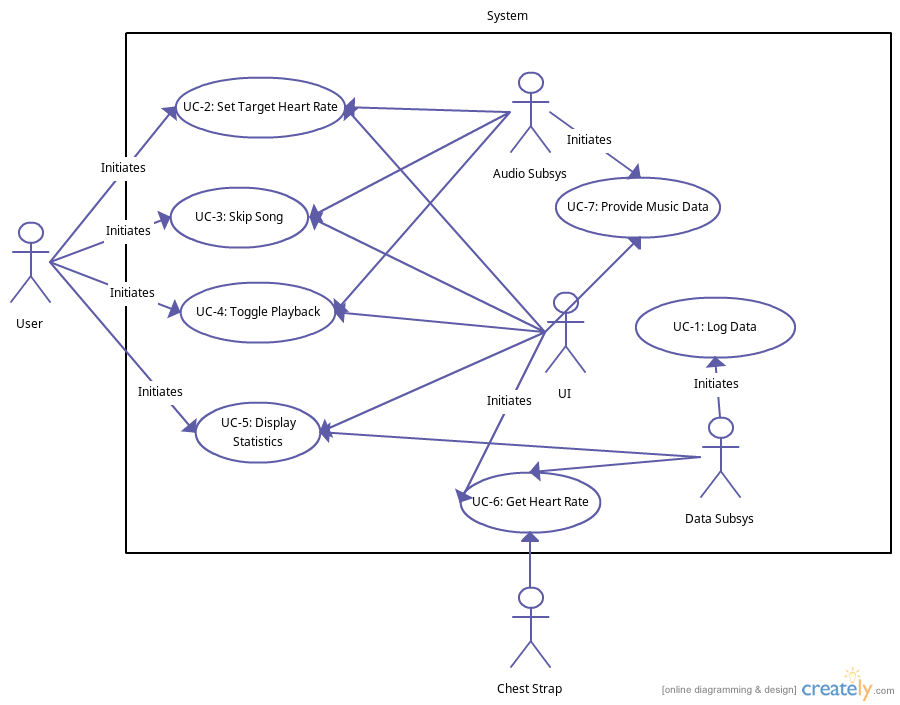
\includegraphics[width=\textwidth]{img/use_case.png}\\
    \caption{Arrows imply participation unless specified}
\end{figure}

\subsection{System Sequence Diagrams}
\begin{figure}[H]
        \centering
        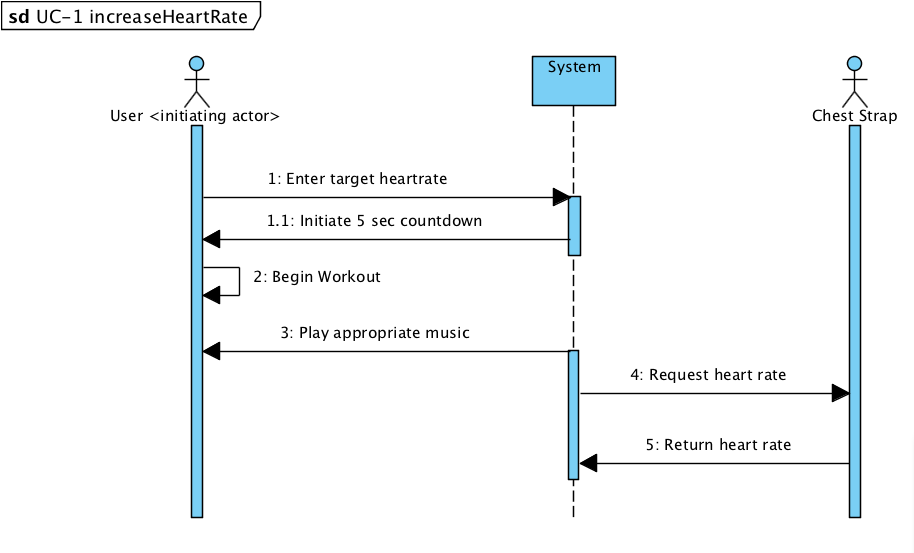
\includegraphics[width=\textwidth]{img/ssd/ssd_uc1.png}\\
\end{figure}

\begin{figure}[H]
        \centering
        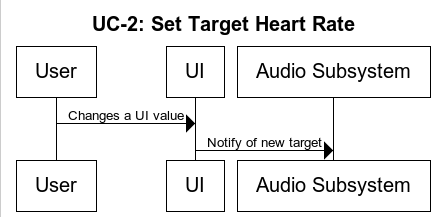
\includegraphics[width=\textwidth]{img/ssd/ssd_uc2.png}\\
        %title UC-2: Set Target Heart Rate
        %User->UI: Changes a UI value
        %UI->Audio Subsystem: Notify of new target
\end{figure}

\begin{figure}[H]
        \centering
        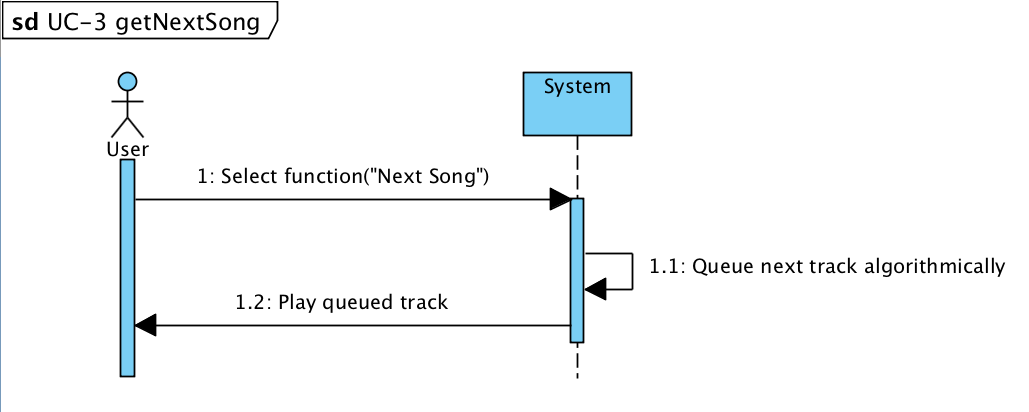
\includegraphics[width=\textwidth]{img/ssd/ssd_uc3.png}\\
\end{figure}
	%title UC-3: Skip the Current Song
	%User->UI: Presses a UI button
	%UI->Audio Subsystem: Notify of necessary skip
	%Audio Subsystem->User: Plays new track

\begin{figure}[H]
        \centering
        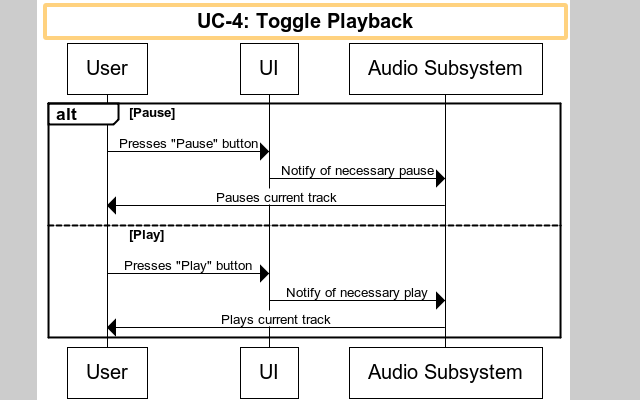
\includegraphics[width=\textwidth]{img/ssd/ssd_uc4.png}\\
\end{figure}
	%title UC-4: Toggle Playback
	%alt Pause
	%    User->UI: Presses "Pause" button
	%    UI->Audio Subsystem: Notify of necessary pause
	%    Audio Subsystem->User: Pauses current track
	%else Play
	%    User->UI: Presses "Play" button
	%    UI-> Audio Subsystem: Notify of necessary play
	%    Audio Subsystem->User: Plays current track
	%end

\begin{figure}[H]
        \centering
        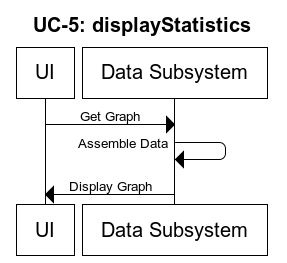
\includegraphics[width=\textwidth]{img/ssd/ssd_uc5.png}\\
\end{figure}
\begin{figure}[H]
	    \centering
        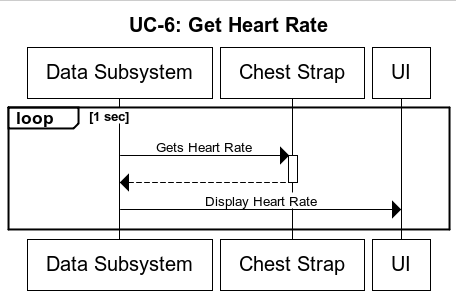
\includegraphics[width=\textwidth]{img/ssd/ssd_uc6.png}\\
        %title UC-6: Get Heart Rate
        %loop 1 sec
        %    Data Subsystem->+Chest Strap: Gets Heart Rate
        %    Chest Strap-->-Data Subsystem:
        %    Data Subsystem->UI: Display Heart Rate
        %end
\end{figure}

\subsection{System Operation Contracts}
{\bf OC-1: Enter Target Heart-rate}
\begin{itemize}
        \item {\bf Precondition: } The application is open to the main screen and prompts the user for input.
        \item {\bf Postcondition: } The system saves the input heart rate and will use it in selecting a song.
\end{itemize}

{\bf OC-2: Select Function("Skip Song")}
\begin{itemize}
        \item {\bf Precondition: } The device is playing a song which needs to be changed.
        \item {\bf Postcondition: } A different song is being played at the same rate at which the previous song was playing.

\end{itemize}

{\bf OC-3: Select Function("Toggle Playback")}
\begin{itemize}
        \item {\bf Precondition: } The system is currently playing a song
        \item {\bf Postcondition: } If the system was playing a song, it stops playing the song and recording the data from the workout. If the system is paused, toggling the playback will cause the system to start playing a song and recording data from the workout.

\end{itemize}

{\bf OC-4: Select Function("Display Statistics")}
\begin{itemize}
        \item {\bf Precondition: } The user has either finished his workout or is in the middle of his workout and would like to see his statistics.
        \item {\bf Postcondition: } The device retrieves the data from the databases, organizes it, and presents it to the user in the form of charts and tables.
\end{itemize}

{\bf OC-5: Select Function("Display Heart Rate")}
\begin{itemize}
        \item {\bf Precondition: } The device should already be monitoring the user's heart rate.
        \item {\bf Postcondition: } The current heart rate is displayed on the screen of the Android application.
\end{itemize}


\subsection{Mathematical Model}
The selection of which track to play requires a mathematical model. At its simplest, this consists of selecting the track with the closest BPM, that is to say minimizing the difference in BPM:
\begin{equation}
  min(\mid target_{BPM} - track_{BPM} \mid)
\end{equation}
If time permits, this simple model can be replaced with a more complex model incorporating Machine Learning to learn which tracks are more effective than others at changing pulse.

\chapter{User Interface Specification}
\section{Preliminary Design}

\subsection{Use Case UC-1: Log Data}
This Use Case doesn't have a User Interface component.

\subsection{Use Case UC-2: Set Target Heart Rate}

\begin{figure}[H]
	\centering
	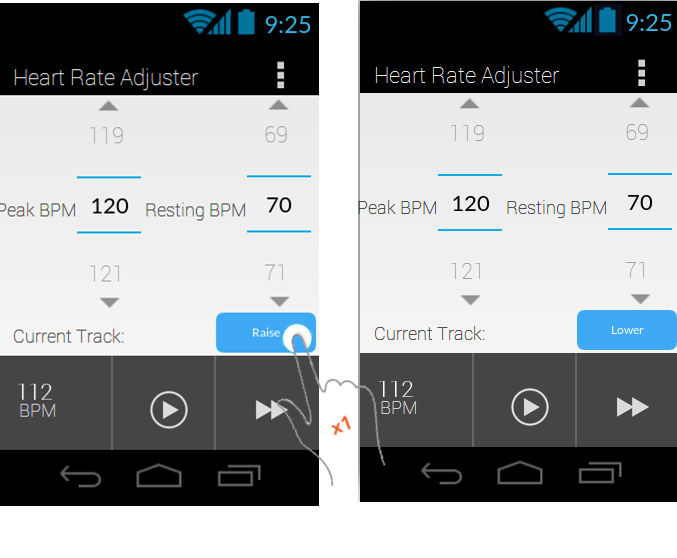
\includegraphics{img/Prelim_Design/PrelimDesign_1.png}\\
\end{figure}

For this Use Case, the user's goal is to select a target heart rate for his workout.
There are two ways a user can trigger this Use Case: modification of the currently active number selector, or pressing the toggle between Raise/Lower.
As seen from the screenshots of our "home" screen above, we seek to minimize user effort in accomplishing his desired goal.
The number selectors are standard Android UI components, so the user is presumably already familiar with their functioning.
Changing the target direction requires only one press, of the Raise/Lower button.
The existence of this button means that, once a user has set their target preferences, they won't need to change the sliders much, reducing the effort of selecting numbers.\\

Once the user has selected a number, the system uses it in playback.

\subsection{Use Case UC-3: Skip Track}

\begin{figure}[H]
	\centering
	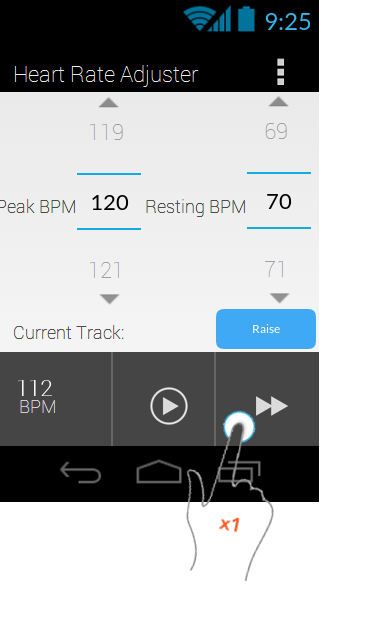
\includegraphics{img/Prelim_Design/PrelimDesign_2.png}\\
\end{figure}

To switch tracks is also very simple. It takes the user one simple tap to achieve his desired outcome. On the provided image of our concept interface, our application appears very similar to a mainstream music player. In the bottom right corner is the double-arrowed fast forward button. The user taps this button to advance to another song, and then the system fulfills that request by running its algorithm and picking out another track from the user's music library. The "Current Track:" label will also be updated accordingly.

\subsection{Use Case UC-4: Toggle Playback}

\begin{figure}[H]
	\centering
	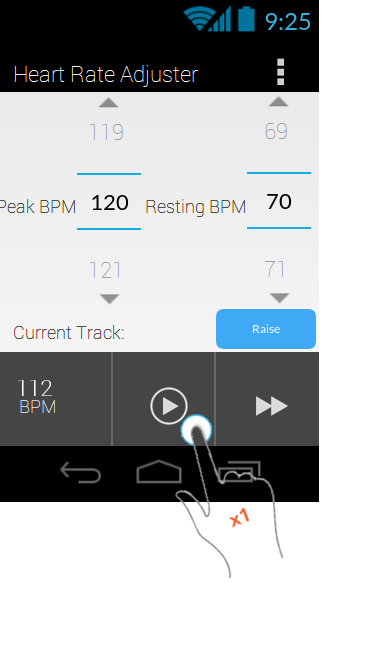
\includegraphics{img/Prelim_Design/PrelimDesign_3.png}\\
\end{figure}

Use Case 4, togglePlayback also proves to be intuitive. Just like most music players, our application has a button located on the bottom center of the screen designed for the purpose of pausing the current song, or playing it, depending on the current state. The user just needs a single tap on the universal play/pause button to achieve his goal of playing or pausing the song.\\

When this is done, if the system was previously playing, the system responds by stopping its collection of heart rate data, and freezing the screen in its current state. 
If the system were not previously playing, the system responds by beginning its collection of heart rate data, and beginning playback.

\subsection{Use Case UC-5: Display Statistics}

\begin{figure}[H]
	\centering
	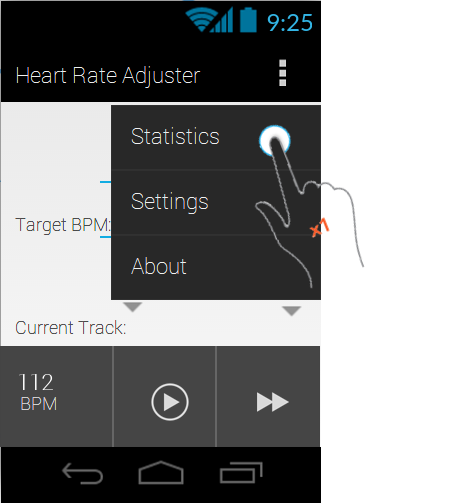
\includegraphics{img/Prelim_Design/PrelimDesign_4.png}\\
\end{figure}

For use case 5, the user desires to view the statistics of his workout.
To simplify the process for the user down to two clicks, we added a menu button in the top right corner of the screen.
After pressing that menu button, a scroll-down menu with three options appears.
The user needs to tap "Statistics" to bring up his workout information.
The system is constantly logging the user data, and compiles a few useful graphs such as heart rate versus time.

\subsection{Use Case UC-6: Get Heart Rate}
\begin{figure}[H]
	\centering
	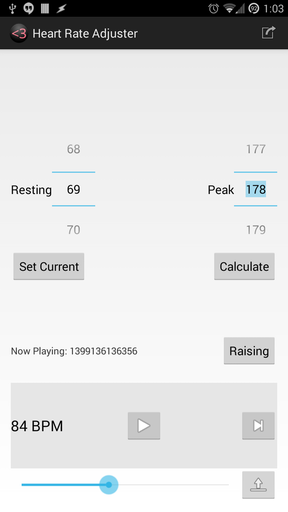
\includegraphics{img/mobile_ui/1.png}\\
\end{figure}

This Use Case requires no user interaction.\\
The UI is updated once a second with the current heart rate read from the chest strap.

\subsection{Use Case UC-7: Provide Music Data}
\begin{figure}[H]
	\centering
	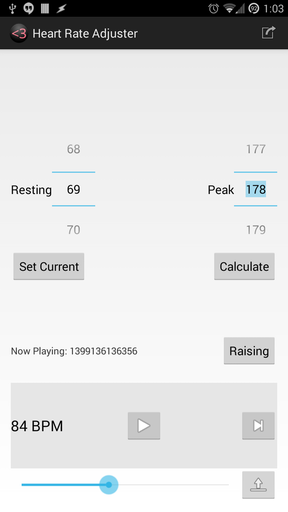
\includegraphics{img/mobile_ui/1.png}\\
\end{figure}

This Use Case requires no user interaction.\\
The UI is updated by the Audio subsystem with the title of the current track.

\section{Effort Estimation}

First we need to calculate the Use Case Points (UCP).

\begin{equation}
UCP = UUCP* TCF *ECF
\end{equation}

Where Unadjusted Use Case Points (UUCPs) are computed as a sum of these two components:

\begin{enumerate}
\item The Unadjusted Actor Weight (UAW), based on the combined complexity of all the actors in all the use cases.
\item The Unadjusted use Case Weight (UUCW), based on the total number of activities (or steps) contained in all the use case scenarios.
\end{enumerate}


\subsubsection{Unadjusted Actor Weight (UAW) and Unadjusted Use Case Weight (UUCW)}
\begin{center}
        \begin{tabular}{|C{3cm}|C{3cm}|C{3cm}|}
                \hline
                        Actor & Complexity & Weight \\
                \hline
                       Users & Complex & 3 \\
                \hline
                       Mobile App & Average & 2 \\
                \hline
        \end{tabular}
\end{center}

\begin{equation}
UAW = 3 + 2 = 5
\end{equation}

Now we reference the Use Case table from 2.5.1 to calculate the UUCW.

\begin{equation}
UUCW = 15 + 15 + 8 + 10 + 12 + 18 = 78
\end{equation}

There the UUCP is:

\begin{equation}
UUCP = 5 + 78 = 83
\end{equation}

\subsubsection{Technical Complexity Factor (TCF)-Nonfunctional Requirements}

Below is a table of Technical complexity factors and their weights.

\begin{center}
        \begin{tabular}{|C{2cm}|C{5cm}|C{1.5cm}|C{2cm}|C{2cm}|}
                \hline
                        Technical Factor & Description & Weight & Perceived Complexity & Calculated Factor \\
                \hline
                        T1 & Friendly interface that the user understands & 2 & 1 & 2 \\
                \hline
                        T2 & Internal processing of heart beat data to music and adjusting BPM shouldn't be too complex & 2 & 3 & 6\\
                \hline
                        T3 & Good Performance & 1 & 2 & 2 \\
                \hline
                        T4 & Security is a minor concern & 1 & 2 & 2 \\
                \hline
                        T5 & No direct access to third parties & 2 & 3 & 6 \\
                \hline
                        T6 & Ease of use is very important & 3 & 3 & 9\\
                \hline   
                        & Technical Factor Total (TFT) & & & 27 \\
                \hline
        \end{tabular}
\end{center}

And $TCF = C1 + C2 \times TFT$, and $C1 = 0.6, C2 = 0.01$, so

\begin{equation}
TCF = 0.6 + 0.01*27 = 0.87
\end{equation}

\subsubsection{Environment Complexity Factor (ECF)}

The environmental factors measure the experience level of the people on the project and the stability of the project. 

\begin{center}
        \begin{tabular}{|C{3cm}|C{5cm}|C{1.5cm}|C{2cm}|C{2cm}|}
                \hline
                        Environmental Factor & Description & Weight & Perceived Impact & Calculated Factor \\
                \hline
                        E1 & Mostly beginners at UML based development & 1.5 & 1 & 1.5 \\
                \hline
                        E2 & Decent familiarity with application problem& 0.5 & 3 & 1.5\\
                \hline
                        E3 & Quite knowledgable about the Object-Oriented approach & 1.5 & 3 & 4.5 \\
                \hline
                        E4 & Somewhat motivated about the problem & 1 & 2 & 2 \\
                \hline
                        E5 & Progamming language proficiency & 2 & 3 & 6 \\
                \hline
                           & Environmental Factor Total (EFT) & & & 15.5 \\
                \hline
        \end{tabular}
\end{center}

Here is the formula to calculate ECF

\begin{equation}
ECF = C1 + C2 * EFT
\end{equation}

Where $C1 = 1.4, C2 = 0.03$.  Therefore we calculate the ECF.

\begin{equation}
ECF = 1.4 + (-0.03*15)=0.965
\end{equation}

So we calculate the final UCP:

\begin{equation}
UCP = 83*0.87*0.965 = 69.68
\end{equation}

If we assume that productivity factor is 30 hours per user case point. The effort estimation would be 2,090.

\chapter{Domain Model}
    \section{Concept Definitions}
		\begin{center}
		\renewcommand{\arraystretch}{1.5}
	        \begin{tabular}[h]{|c|c|c|}
	           \hline
	           Responsibility & Type & Concept\\
	           \hline
	           Pairing/communicating with HRM & D & HRM manager\\
	           \hline
	           Retrieve logged data & D & log retriever\\
	           \hline
	           Musical Playback & D & music playerbacker\\
	           \hline
	           Logging tracks as they are played & D & track logger\\
	           \hline
	           Queue Next Track(s) & D & track queuer\\
	           \hline
	           Listen for user input & D & general UI\\
	           \hline
	           Graphically displaying music information & D & playback view\\
	           \hline
	           Graphically displaying heart rate info & D & heart beat view\\
	           \hline
	           Graphically displaying current workout data & D & workout view\\
	           \hline
	           Graphically displaying previous workout data & D & history view\\
	           \hline
	           Data store for workout data & K & workout store\\
	           \hline
	           Data store for music metadata & K & metadata store\\
	           \hline
	           Data store for music files & K & music store\\
	           \hline
	       \end{tabular}
		\end{center}
	   
    \section{Association Definitions}
		
		\begin{center}
			\renewcommand{\arraystretch}{1.5}
	        \begin{tabular}{| m{0.25\textwidth} | m{0.4\textwidth} | c |}
	            \hline
	            Concept Pair & Association Description & Association Name\\
	            \hline
	            music playerbacker $\leftrightarrow$ metadata store & music playerbacker retrieves information about the current track from metadata store & data retrieval\\
				\hline
	            history view $\leftrightarrow$ workout store & history view retrieves data about previous workouts from the workout store & data retrieval\\
				\hline
	            track logger $\leftrightarrow$ music playerbacker & tracks played by music playerbacker are logged by track logger & data logging\\
				\hline
	            music playerbacker $\leftrightarrow$ track queuer & music playerbacker retrieves the next track from the track queuer & data retrieval\\
				\hline
	            music playerbacker $\leftrightarrow$ playback view & playback view displays information based on the data in music playerbacker & human data interface\\
				\hline
	            hrm manager $\leftrightarrow$ general UI & general UI pairs and reports hrm status based on hrm manager & human data interface\\
				\hline
	            heart beat view $\leftrightarrow$ hrm manager & retrieves and displays heart rate data from the hrm manager & human data interface\\
				\hline
	            log retriever $\leftrightarrow$ workout store & log retriever fetches logs from the workout store and barks at the mailman & data logging\\
				\hline
	            music playerbacker $\leftrightarrow$ music store & music playerbacker plays songs from the music store & data retrieval\\
				\hline
	        \end{tabular}
		\end{center}

    \section{Attribute Definitions}
		\begin{center}
			\renewcommand{\arraystretch}{1.5}
	        \begin{tabular}[h]{| c | c | m{0.4\textwidth} |}
	            \hline
	            Concept & Attribute & Attribute Definition\\
	            \hline			
	            HRM manager & \multirow{3}{*}{data logging} & \multirow{3}{0.4\textwidth}{Data logging has to with the storage or retrieval of logged data or the logging of data.} \\
				\cline{1-1}
	            log retriever & & \\
				\cline{1-1}
	            track logger & & \\
				\hline
	            music playerbacker & \multirow{7}{*}{human data interface} & \multirow{7}{0.4\textwidth}{Human data interfaces deal with the interaction between the user and the data.}\\
				\cline{1-1}
	            track queuer & &\\
				\cline{1-1}
	            general UI & &\\
				\cline{1-1}
	            playback view &&\\
				\cline{1-1}
	            heart beat view & &\\
				\cline{1-1}
	            workout view & & \\
				\cline{1-1}
	            history view & &\\
				\hline
	            workout store & \multirow{3}{*}{data storage} & \multirow{3}{0.4\textwidth}{Data storage deals with the storage of the data.}\\
				\cline{1-1}
	            metadata store & &\\
				\cline{1-1}
	            music store & &\\
	            \hline
	        \end{tabular}
		\end{center}

    \section{Tracability Matrix}
		\begin{center}
			\renewcommand{\arraystretch}{1.5}
	        \begin{tabular}[h]{|c|c|c|c|c|c|c|c|c|c|c|c|c|c|}
		        \hline
		        & \rotatebox{90}{HRM manager} & \rotatebox{90}{log retriever} & \rotatebox{90}{track logger} & \rotatebox{90}{music playerbacker} & \rotatebox{90}{track queuer} & \rotatebox{90}{general UI} & \rotatebox{90}{playback view} & \rotatebox{90}{heart beat view} & \rotatebox{90}{workout view} & \rotatebox{90}{history view} & \rotatebox{90}{workout store} & \rotatebox{90}{metadata store} & \rotatebox{90}{music store}\\
				\hline
		        UC-1 & X &  &  & X & X & X & X &  &  &  & X & X &\\
				\hline
		        UC-2 & X &  &  & X & X & X & X &  &  &  & X & X &\\
				\hline
		        UC-3 &  &  & X & X & X & X & X &  &  &  &  & X & X\\
				\hline
		        UC-4 & X &  &  & X &  & X & X & X & X &  & X &  &\\
				\hline
		        UC-5 &  & X &  &  &  & X &  &  &  & X & X &  &\\
				\hline
		        UC-6 & X &  &  &  &  & X &  & X & X &  & X &  &\\
				\hline
	        \end{tabular}
		\end{center}
\chapter{Plan of Work}

Looking ahead at some of the due dates in the near future, our group will probably be mixing documentation with development during the course of March. Up until now, we have been primarily working on laying the foundations of our project. We have been examining customer and system requirements and extracting specifications from them. We have been envisioning preliminary design as well as analyzing user estimation. We have derived our domain and mathematical models. 
In the upcoming weeks, we will be working on some UML diagrams to make our lives a lot easier when we begin to code. We will complete the sequence and class diagrams to help us understand exactly which attributes and classes we need to account for. We will also design our system architecture to further our understanding on how each of the components of our system interface and communicate with each other. We will identify any data algorithms or structures needed to store the information generated by the phone and the heart rate monitor. Finally, we will continue to revise our designs and implementations from our previous iteration and construct tests to ensure that our system works as planned.
By doing this preliminary design and analysis in conjunction with the upcoming deliverables, we will develop a solid understanding of what pieces of software actually need to be written. We will have a snapshot of our system and hopefully foresee some of the problems that might have occurred had we rushed straight into coding.
The included Gantt chart serves as a visual roadmap of our project plan.

\section{Gantt Chart}


\begin{figure}[H]
	\centering
	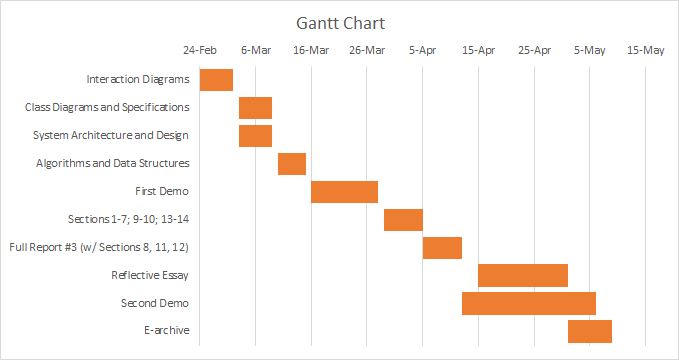
\includegraphics{img/Gantt_Chart.png}\\
	\caption{Our Gantt Chart details our plan of work in the upcoming weeks leading up the second report, and also lists our hopes for the second iteration.}
\end{figure}


\section{Product Ownership}
Our team will be divided into three smaller sub-teams of two individuals each, the pairings listed below. Each sub-team will be responsible for developing a specific sub-product during the bulk of their time. Upon completion of a significant portion of work, they will provide a brief description of their activity before they push it to our Github repository. In addition to documentation, they will also include the necessary UML diagrams, charts, algorithms, and source code. Every week, or at least once before each deliverable, we will meet together for 1-3 hours during a timeframe determined by a combination of GroupMe and When2meet. During the meeting, we will have a specific agenda that primarily involves the week's progress and upcoming deliverable. Our discussion will probably be centered along the following questions: 1) What did you work on this past week? 2) What do you plan on working on next week? 3) Are there any revisions that need to be made to the project? Every week, a team member will take the lead for the next deliverable to ensure that everything is on time.

\begin{itemize}
	\item Revan and Tae-Min will work on the general user interface of the mobile application. They will design the layout and basic functionality of the Android app, and set up the communication protocol between the heart rate monitor and the phone. 
	\item Kenny and Samani will work on the music aspect of the mobile application. They will study music playback features such as track selection and queuing to provide customers with a seamless music player experience. They will also be responsible for the nuances of audio playback such as crossfading transitions and tempo adjustments.
	\item Jon and Nikhil will work on the data logging faculties that are necessary to provide the user with feedback about his/her workout. They will work with a server that captures heart rate and music data from the phone and possibly directly from the heart rate monitor. They will determine how to process this information on the server and create customizable graphical displays for user's to view.
\end{itemize}


\section{Breakdown of Responsibilities}

\begin{center}
        \begin{tabular}{|C{2cm}|C{6cm}|C{3cm}|C{3cm}|}
                \hline
                         & \textbf{Past} & \textbf{Present} & \textbf{Future}  \\
                \hline
                        \textbf{Jonathan} & Problem Statement, Enumerated Functional Requirements, Preliminary Design, References & Plan of Work & Project Management, Interaction Diagrams, Class Diagrams \\
                \hline
                        \textbf{Kenny} & User Effort Estimation & Domain Analysis & System Architecture and System Design \\
                \hline
                        \textbf{Nikhil} & Enumerated Nonfunctional Requirements, Use Cases (Casual Description, Traceability Matrix, Fully-Dressed Description) & System Operation Contracts & Project Management, Interaction Diagrams, Class Diagrams  \\
                \hline
                        \textbf{Revan} & On-Screen Appearance Requirements, Use Case Diagrams & Mathematical Model & Class Diagrams, System Architecture and System Design \\
                \hline
                        \textbf{Samani} & System Sequence Diagrams & Domain Analysis & System Architecture and System Design \\
                \hline
                        \textbf{Tae-min} & Glossary of Terms, Stakeholders, Actors, Goals & System Operation Contracts & Algorithms and Data Structures \\
                \hline   
                       
        \end{tabular}
\end{center}

\chapter{Interaction Diagrams}
	
\begin{figure}[H]
	\centering
	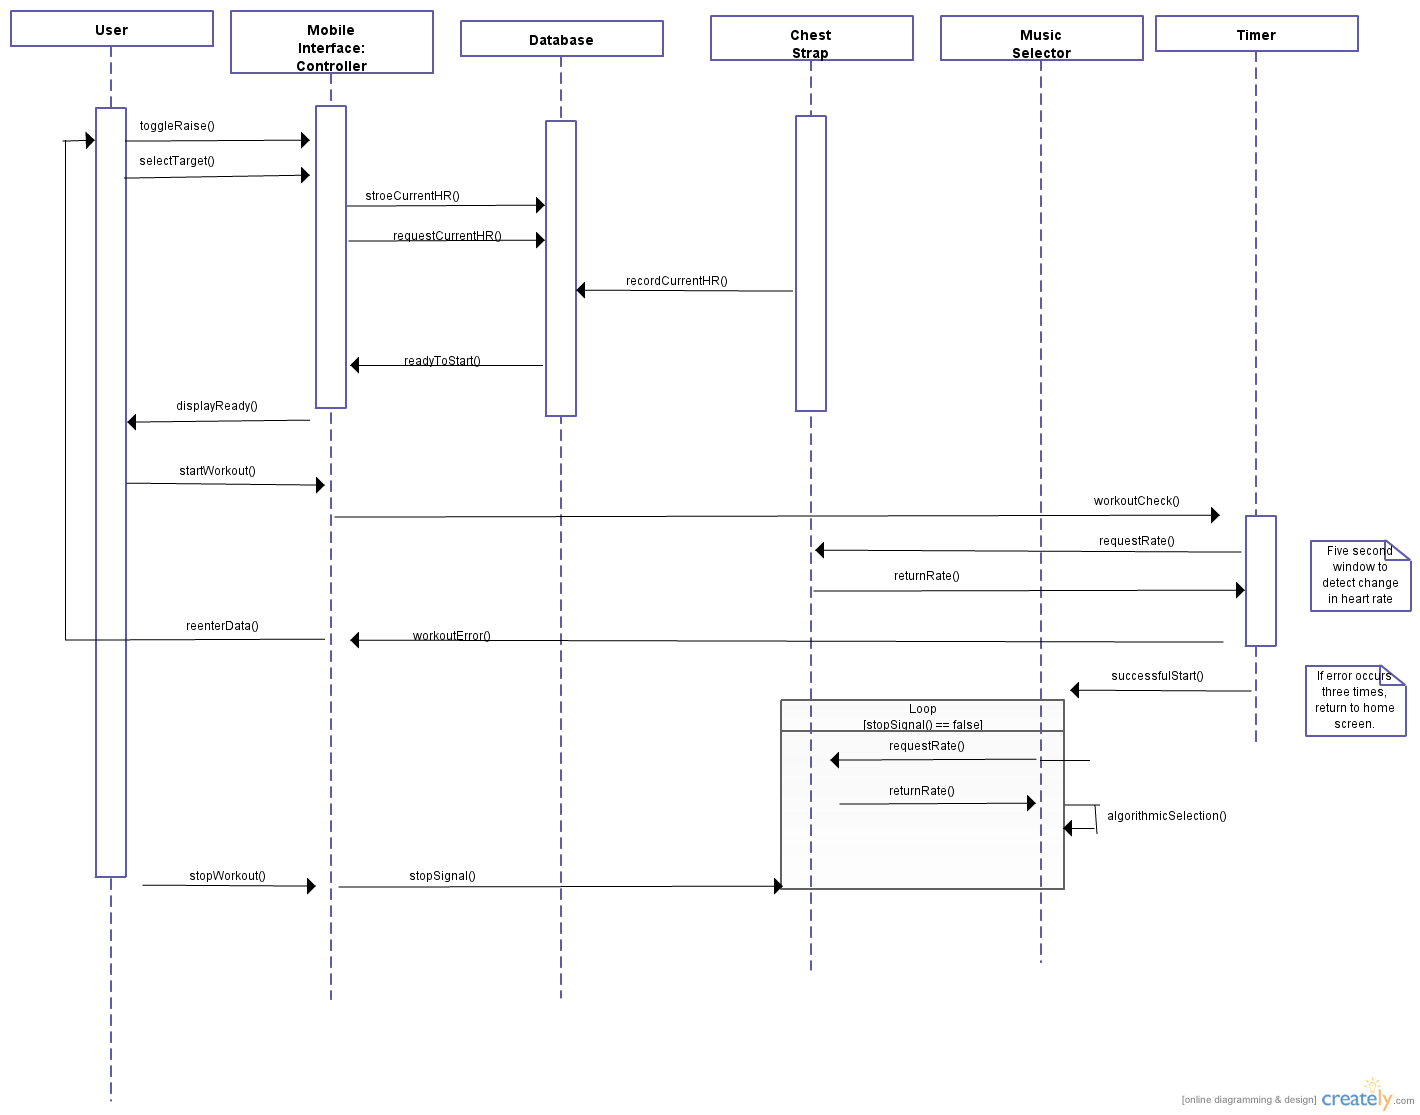
\includegraphics[scale=.35]{img/Interaction_Diagrams/newUC1.png}\\
	\caption {Interaction diagram for the increaseHeartRate case} 
\end{figure}


Since our first two use cases are very similar, we only include the interaction diagram for UC-1, increaseHeartRate. Again, the user toggles the ``raise'' button from the home screen and scrolls to the desired BPM. The database manager coordinates with the heart rate monitor and uses its own algorithm to determine the appropriate song for the music player to play for the user. Then, it waits five seconds for the user to begin his workout. Upon playback, the database manager continuously receives the user's current BPM and makes adjustments to the song's tempo accordingly.

\begin{figure}[H]
	\centering
	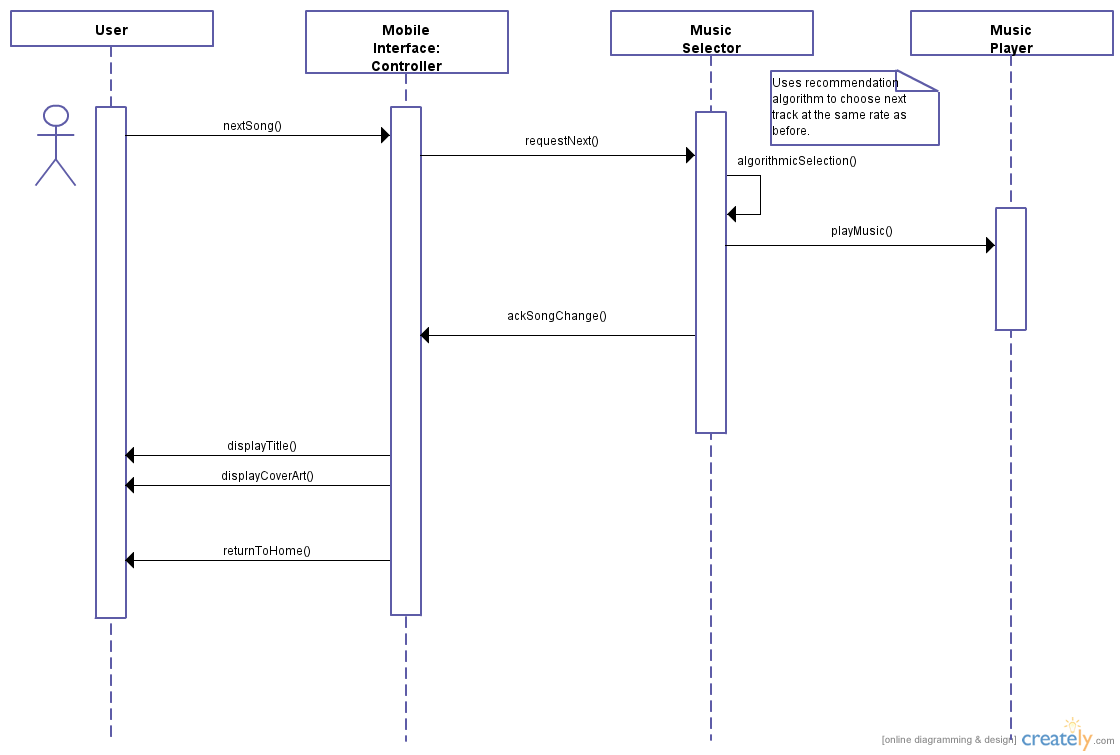
\includegraphics[scale=.40]{img/Interaction_Diagrams/newUC3.png}\\
	\caption {Interaction diagram for getNextSong()} 
\end{figure}

For our third use case, the user's goal is to listen to another song. Similar to the ``skip'' button on most standard music players, we included a double fast-forward arrow for users' convenience. When pressed, the controller immediately contacts the database manager. The database manager selects another track based on its song-selection algorithm for the music player to play. (If the user is currently trying to change his/her heart rate, the database manager will take that into count and select a song of a similar speed.) It also returns the cover art and new song title for the mobile interface to display.

\begin{figure}[H]
	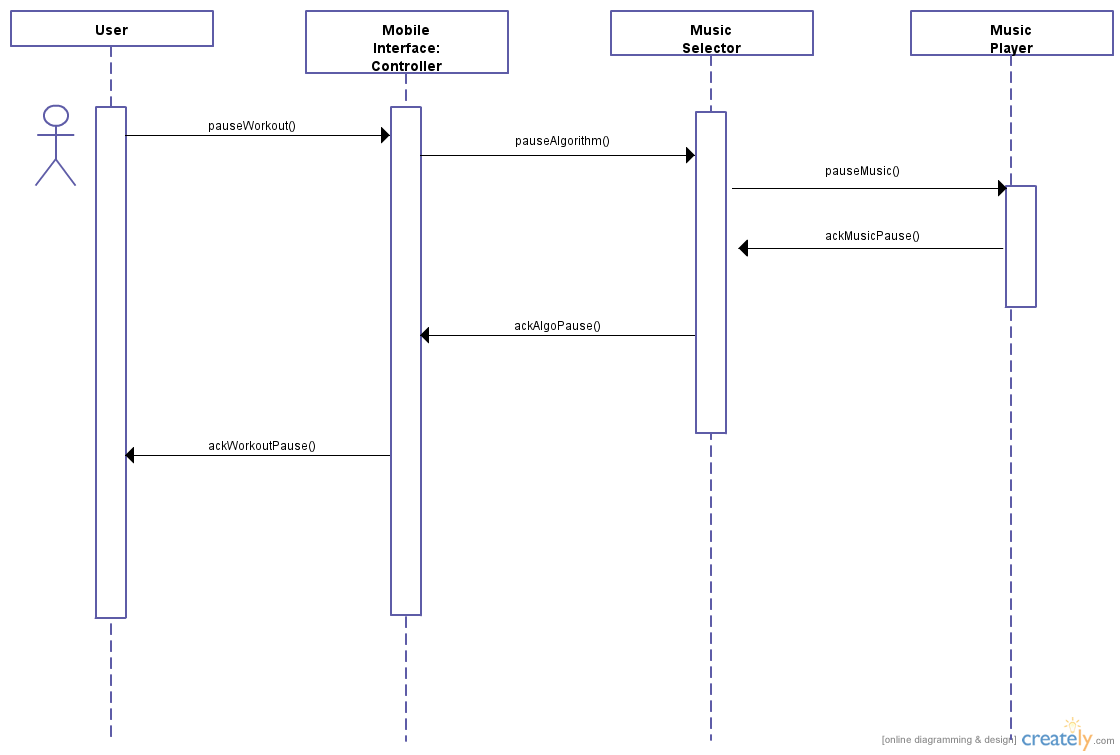
\includegraphics[scale=.40]{img/Interaction_Diagrams/newUC4.png}\\
	\caption {Interaction diagram for togglePlayback()} 
\end{figure}

Our togglePlayback sequence is fairly simple. The user initiates the request by tapping the play/pause button. Then the controller informs the database manager to store the current state settings for future use, and the database manager proceeds to stop recording data and allows the music player to stop the song. The mobile display also updates accordingly.

\begin{figure}[H]
	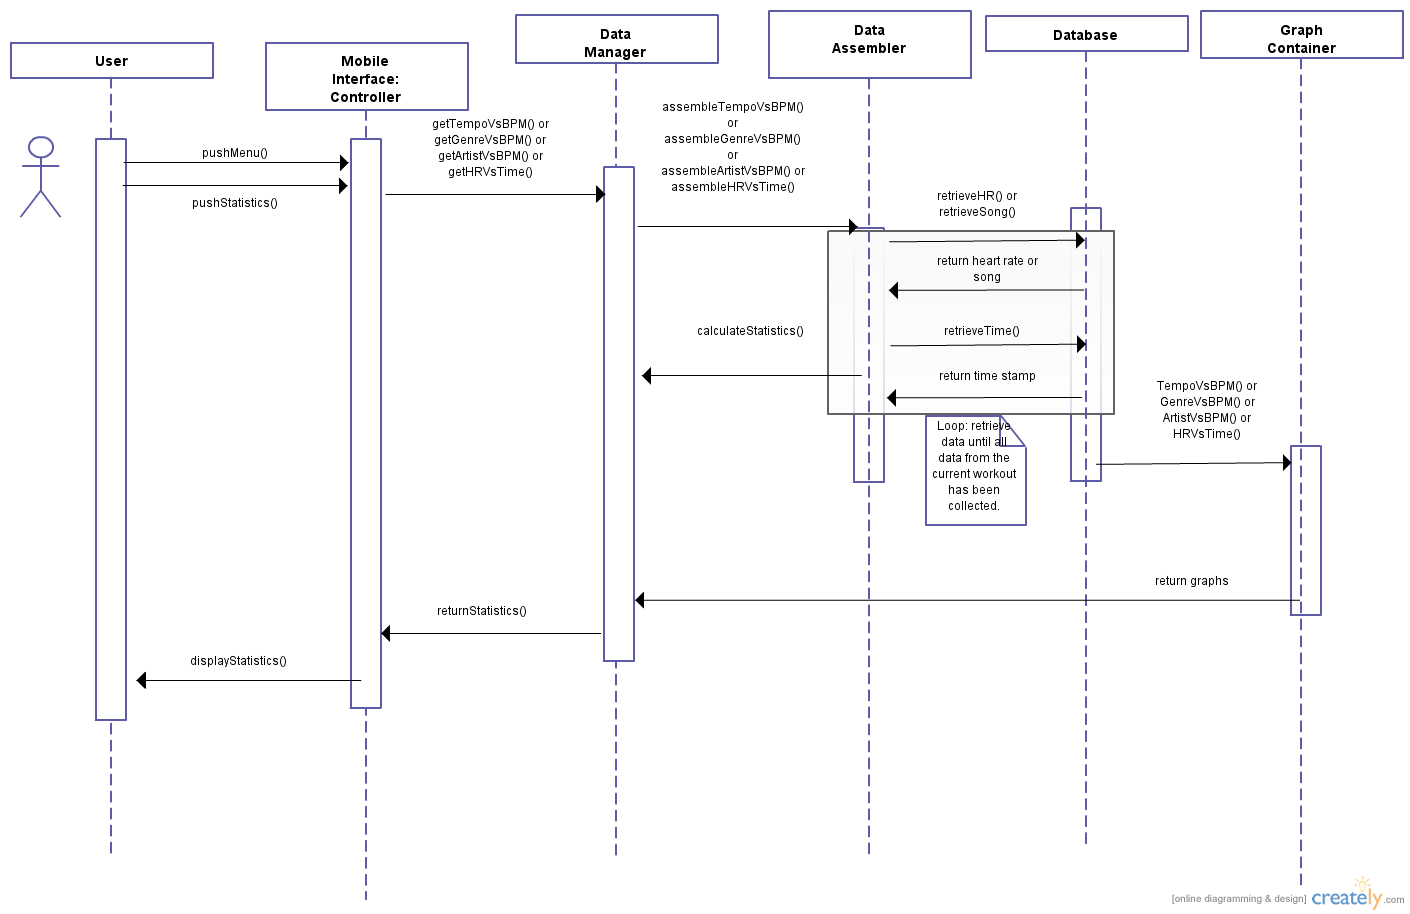
\includegraphics[scale=.40]{img/Interaction_Diagrams/displayStatistics.png}\\
	\caption {Interaction diagram for displayStatistics()} 
\end{figure}
In UC-5, getStatistics, the user begins with two button presses to achieve their goal. First, they bring up the menu button in the top right hand corner and then press ``Statistics'' from the dropdown. The controller passes this request to the database manager, which quickly retrieves and updates the data. Then, it calculates statistics, creates some graphs, and then returns the output to the controller to display. (Note that the user must select from the options available in order to view his workout history.)

\begin{figure}[H]
	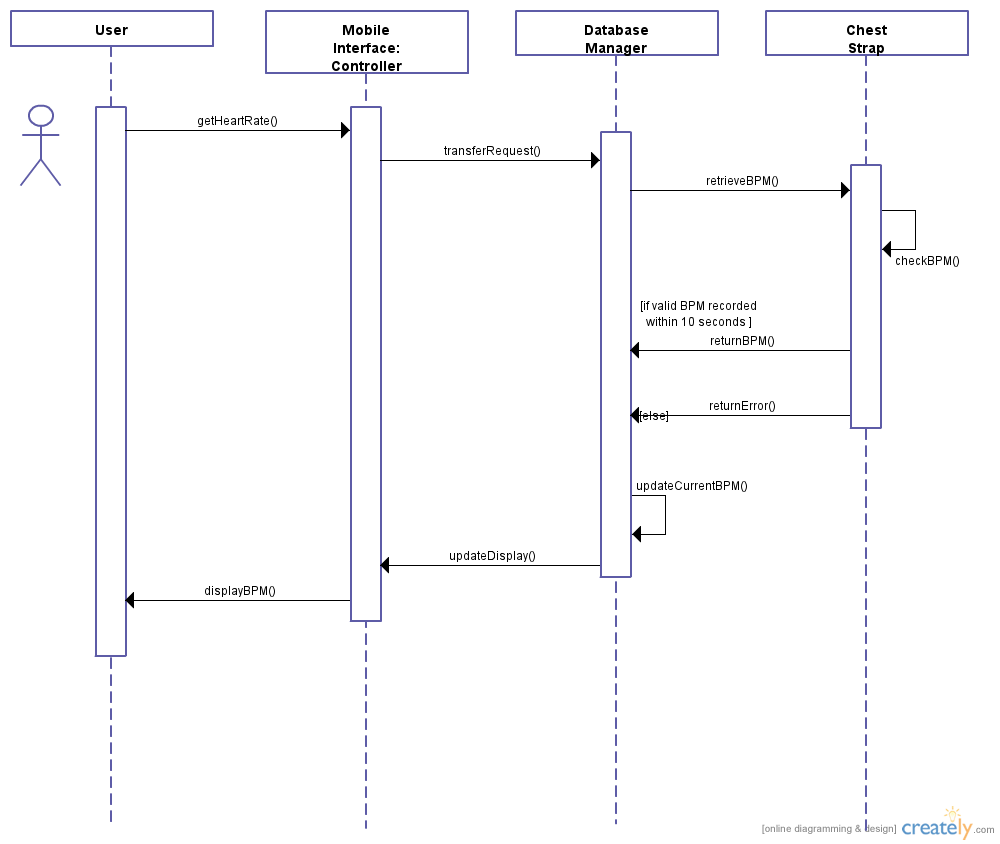
\includegraphics[scale=.40]{img/Interaction_Diagrams/newUC6.png}\\
	\caption {Interaction diagram for getHeartRate()} 
\end{figure}

UC-6, getHeartRate is very similar to UC-5. This use case is also applicable for UC-1, because the Heart Rate is important, needing to be determined continuously. The controller takes the request from the user and passes it to the database manager to handle. The database manager then takes the current BPM value from the Heart Rate Monitor and updates the value for the mobile interface to display to the user. 


\section{Alternate Scenarios}
\begin{figure}[H]
	\centering
	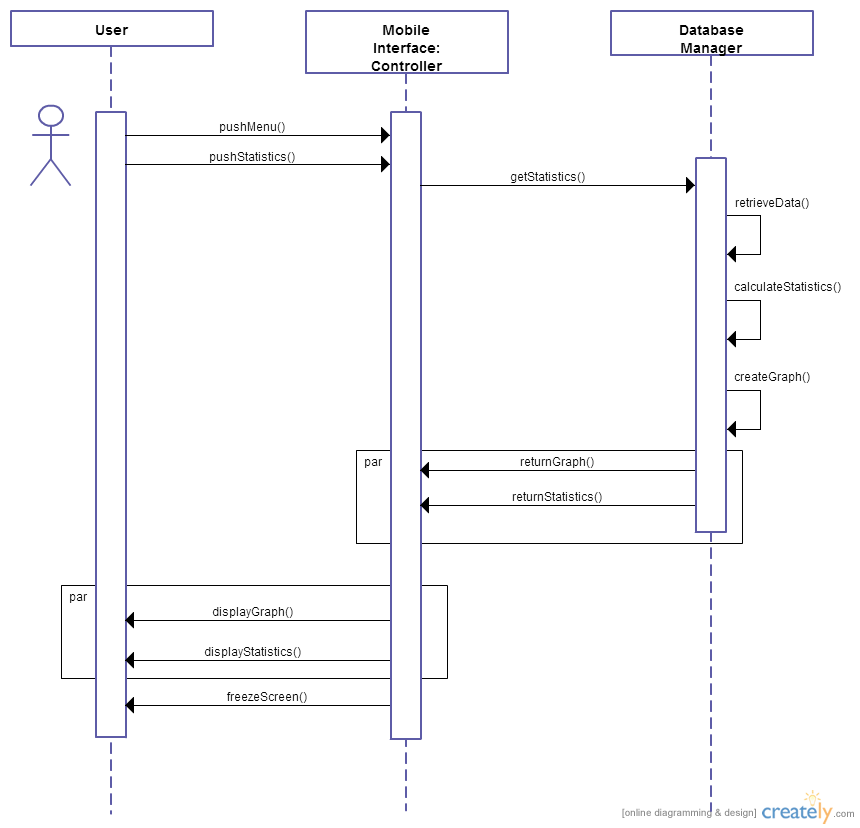
\includegraphics[scale=.30]{img/Interaction_Diagrams/UC-5_getStatistics.png}\\
	\caption {Alternate interaction diagram for getStatistics without the Statistics Generator Object}
	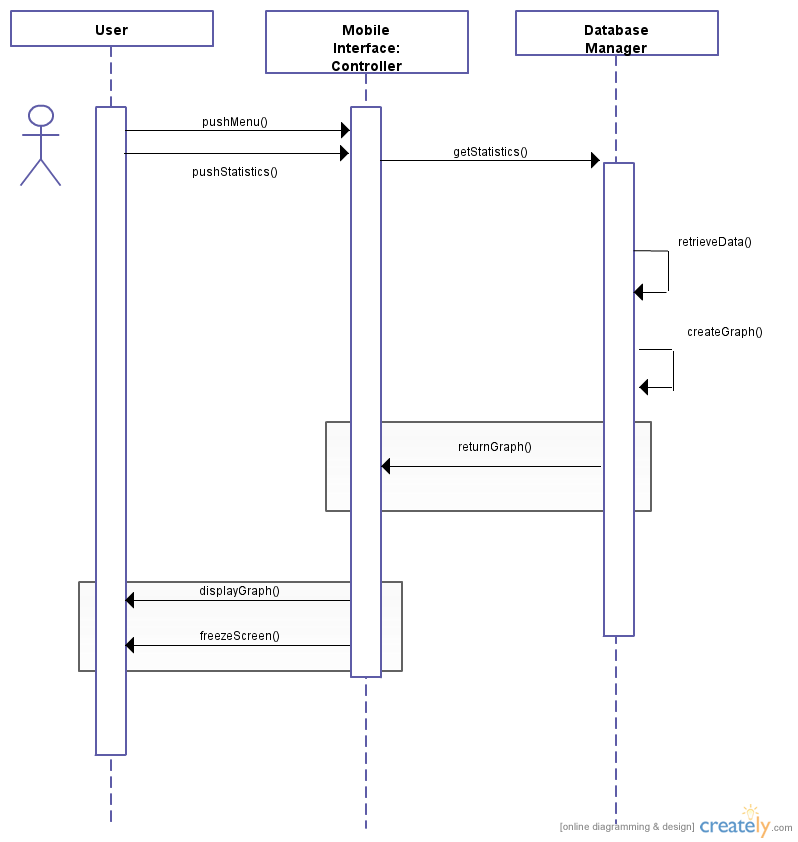
\includegraphics[scale=.30]{img/Interaction_Diagrams/getStatisticsAlternateGraphs.png}\\
	\caption {Alternate interaction diagram for getStatistics() using getGraphs()} 
\end{figure}

\begin{figure}[H]
	\centering
	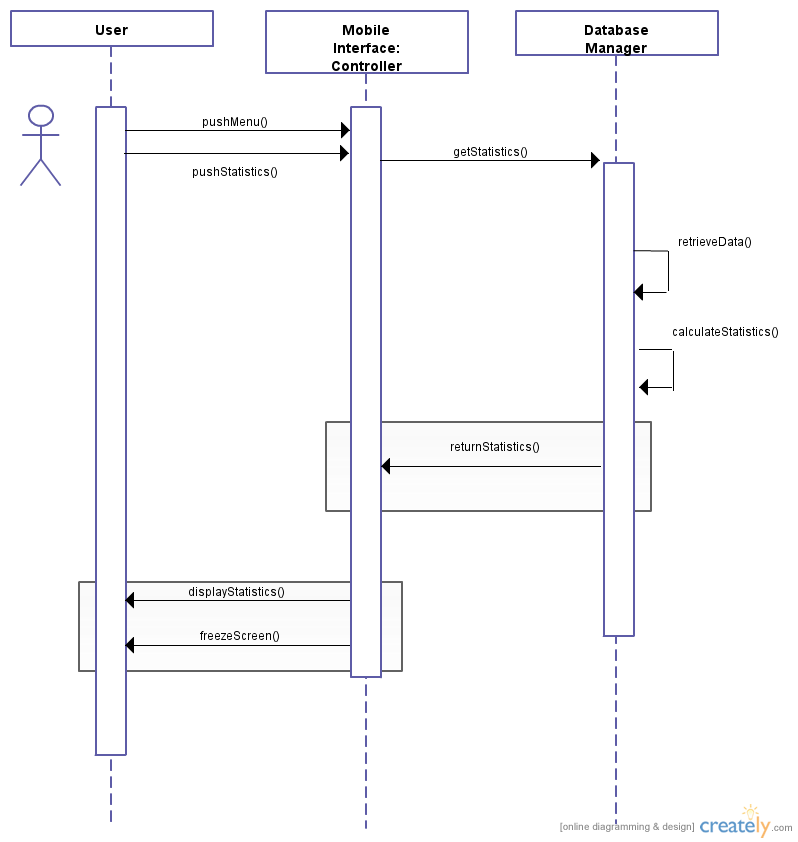
\includegraphics[scale=.30]{img/Interaction_Diagrams/getStatisticsAlternateNumbers.png}\\
	\caption {Alternate interaction diagram for getStatistics() using calculateStatistics()} 
\end{figure}




Alternate scenarios could occur mainly during the getStatistics() use case. Here, the user can select which particular graphs or data he may want to see. In the original diagram, a dedicated Statistics Generator object was created to handle the organization and creation of all statistics. This object greatly simplifies the displayStatistics() case because all the calculations are done outside of the database. However, this is not the only way to solve the case, with the alternative solution being that the statistics are generated directly by the database. Advantages of this are that there is no need to transfer the data between two objects and worry about the communication scheme between them. Also, the time needed to flesh out an entirely new class to handle the calculations would be eliminated. Three different scenarios of keeping the statistics-generation functionality are displayed above. In these diagrams, it is assumed that the user has selected all the options available for getStatistics(), and thus all the graphs and statistics available to the database are displayed to the user. This may not always be the case, as some users may prefer to see graphs only, or numbers only. Some users would like to see a certain combination of both. Thus, our alternate scenarios for the getStatistics() consist of various combinations of all the different display options. For simplicity, only the cases for displaying only graphs and for displaying only numbers are shown in separate interaction diagrams. 

Although keeping the statistics-generation functionality can be contained entirely within the database, we implemented it within a Statistics Generator object. This decision was made to keep consistency with the High Cohesion and Low Coupling Principles. If we hadn`t made the separation, then the database would have too many responsibilities to take care of. By creating a dedicated Statistics Generator object, the statistics can be fully fleshed out and managed without having to worry about other responsibilities.

\section{Design Patterns}

This project was developed through a mainly object-oriented approach. We were able to boil our system down to a few, distinct actors, and an object-oriented approach seemed appropriate to model our system. As evidenced by the interaction diagrams, there are five main actors: the user, the mobile interface, the database, the music player, and the heart rate monitor. Each of these actors has a specific set of actions that they can perform, and these actions are not very tightly coupled to those of other actions in the system. For example, the music player is designated to solely play the music on the device. It does not have access to the music algorithm or the heart rate; its sole job is to respond to requests about playing or pausing the music. Similarly, the database manager is solely responsible for manipulating data and handling requests. These characteristics are prime examples of the High Cohesion principles, because each actor in the system has its own specific tasks, and the respective actors are designed to that their tasks are carried out very well. We acknowledge that some of the actors are more important than the others, such as the database manager and the mobile interface, but this is out of necessity. The user interacts directly with the interface, and the interface talks directly to the database in most cases. The other objects in the system are more supplementary in the sense that they carry out the commands given to them by the database-mobile-interface pair. Although there is some communication between the different objects, the communication has been designed such that each method call is specific, efficient, and effective. This cuts back on unnecessary communication between the objects and allows for the system to be optimized. The Low Coupling Principle requires that objects should ``not take on too many communication responsibilities'', and our design fulfills the requirement because we have minimized the number of interactions to just the necessary ones. All in all, our object-oriented design encompasses aspects from both the High Cohesion and Low Coupling principles, and creates and effective solution to the heart rate monitoring problem.

\section{Assignment of Responsibilities}

A prime example can be found in UC-4, togglePlayback. Each object submits a request to the next object in line before reaching the Music Player, which is supposed to fulfill the ``pause'' function. At this point, the interactions start coming back. It is clearly seen that each object in this example transmits at most two messages, and no object performs more than a single computation. A similar theme exists in UC-6, getHeartRate. Each object essentially sends one message and receives one message. Furthermore, each object does not need to fulfill more than two active responsibilities. We believed that by distributing the workload for each object through the High Cohesion Principle and the Low Coupling Principle, we would be reaching the best balance.
The Expert Doer Principle was not followed as closely because the communication links of the objects we used are a bit longer. In our design, the ``one who knows'' often passes on the knowledge to another object that ``needs to know'' before the task is actually fulfilled. For instance, the Database Manager often causes the Controller to update the display and show the user rather than directly communicating with the user. Basically, our Controller and Database Manager are both extremely important, so oftentimes, they both end up with most of the implementation details.

\chapter{Class Diagram and Interface Specification}

\section{Class Diagram}
\subsection{Class Diagram for Data Management}

\begin{figure}[H]
	\centering
	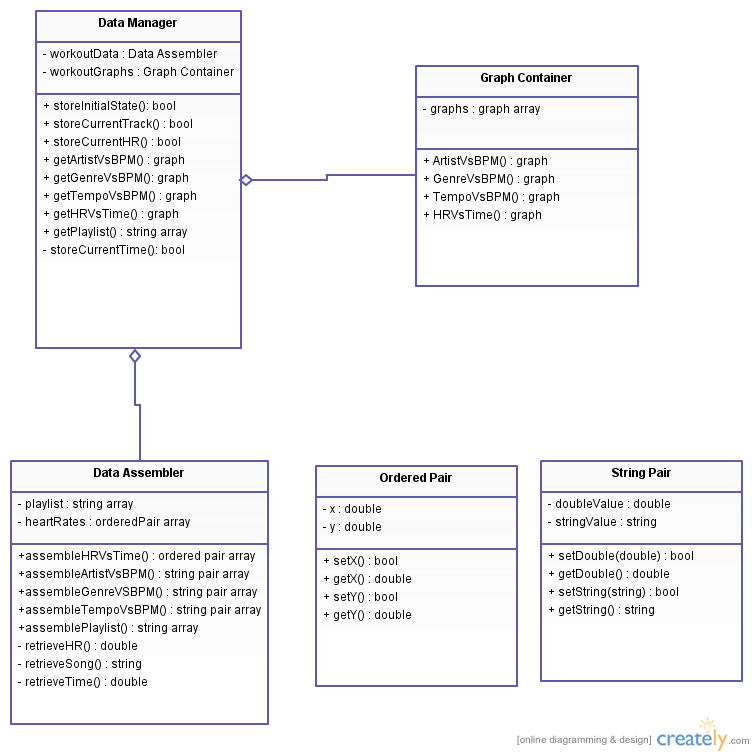
\includegraphics[scale=.55]{img/Class_Diagrams/dataManagement.png}\\
	\caption {Class relationship for managing data}
\end{figure}

\section{Data Types and Operation Signatures}
\begin{center}
        \begin{tabular}{|C{15cm}|}
                \hline
                        \textbf{Data Manager}\\
                \hline
                        \begin{flushleft}
                                \textbf{Variables:} \\
                        \end{flushleft}
                                \begin{itemize}
                                        \item workoutData: Data Assembler. This is a Data Assembler object which stores the data points retrieved from storage. It also stores the songs and their metadata.
                                        \item workoutGraphs : Graph Container. This is a Graph Container object which stores the different graphs that were requested by the User Interface.
                                \end{itemize} \\
                        \hline
                        \begin{flushleft}
                                \textbf{Functions:} \\
                        \end{flushleft}
                                \begin{itemize}
                                        \item storeInitialState(double initialRate, double targetRate) : bool. This function stores the initial state of the system, which is captured in the form of the user's initial heart rate and the target heart rate.
                                        \item storeCurrentTrack(string song) : bool. This function is used by the Music Module to store the current track being played. This information is later used for the playlist.
                                        \item storeCurrentHR(double heartRate) : bool. This function is used to store the current heart rate into the data storage. It is used by the User Interface while the user is working out with the system.
                                        \item getArtistVsBPM() : graph. This function will access the data stored in the Data Assembler and create a histogram displaying the artist who's songs were played most often at different BPMs. The Data Manager will select the appropriate graph from the Graph Container and return it to the UI.
                                        \item getGenreVsBPM() : graph. This function will create a histogram of the most frequent genres at different BPMs. The data will be accessed from the Data Assembler and plotted by the Graph Container. The final graph will be selected by the Data Manager from the Graph Container
                                        \item getTempoVsBPM() : graph. This function will return a graph of the music's tempo versus the user's BPM.
                                        \item getHRvsTime() : graph. This function will return a graph of the user's heart rate over time.
                                        \item getPlaylist(): string array. This function will return an array of the music that was played during the workout.
                                        \item storeCurrentTime() : bool. This is an auxiliary function which stores the current system time in the data storage every time storeCurrentHR() is called. It will associate the time with the current heart rate.
                                \end{itemize}\\
                        \hline
        \end{tabular}
\end{center}

\begin{center}
        \begin{tabular}{|C{15cm}|}
                \hline
                        \textbf{Data Assembler} \\
                \hline
                        \begin{flushleft}
                                \textbf{Variables:} \\
                        \end{flushleft}
                                \begin{itemize}
                                        \item playlist: string array. This variable will store the names of the songs that were played during the workout.
                                        \item heartRates: Ordered Pair array. This variable will store the retrieved data points in ascending order.
                                \end{itemize} \\
                        \hline
                        \begin{flushleft}
                                \textbf{Functions: } \\
                        \end{flushleft}
                                \begin{itemize}
                                        \item assembleHRVsTime() : ordered pair array. This function assembles the data for an HR vs Time graph.
                                        \item assembleArtistVsBPM() : string pair array. This function assembles the data for an Artist vs BPM table.
                                        \item assembleGenreVsBPM() : string pair array. This function assembles the data for a Genre vs BPM table.
                                        \item assembleTempoVsBPM() : string pair array. This function assembles the data for a Tempo vs BPM table.
                                        \item assemblePlaylist() : string array. This function assembles the music playlist.
                                        \item retrieveHR() : double. This function retrieves a heart rate from the data storage.
                                        \item retrieveTime() : double. This function retrieves a time from the data storage.
                                        \item retrieveSong() : string. This function retrieves a song name from data storage.
                                \end{itemize} \\
                        \hline
        \end{tabular}
\end{center}

\begin{center}
        \begin{tabular}{|C{15cm}|}
                \hline
                        \textbf{Graph Container} \\
                \hline
                        \begin{flushleft}
                                \textbf{Variables:} \\
                        \end{flushleft}
                                \begin{itemize}
                                        \item graphs : graph array. This variable contains an array of the different graphs that were requested by the User Interface.
                                \end{itemize} \\
                        \hline
                        \begin{flushleft}
                                \textbf{Functions: } \\
                        \end{flushleft}
                                \begin{itemize}
                                        \item ArtistVsBPM(Data Assembler workoutData) : graph. This function takes the names of the artists and heart rates stored in the Data Assembler and graphs them against each other.
                                        \item GenreVsBPM(Data Assembler workoutData) : graph. This function graphs the genre of the music versus the user's heart rate using the data from workoutData.
                                        \item TempoVsBPM(Data Assembler workoutData) : graph. This function graphs the tempo of the music versus the user's heart rate using the workoutData object.
                                        \item HRVsTime(Data Assembler workoutData) : graph. This function graphs the user's heart rate versus time using the workoutData object.
                                \end{itemize} \\
                        \hline
        \end{tabular}
\end{center}


\begin{center}
	\begin{tabular}{|C{15cm}|}
		\hline
			\textbf{Ordered Pair} \\
		\hline
			\begin{flushleft}
				\textbf{Variables: }\\
			\end{flushleft}
				\begin{itemize}
					\item x : double. This variable stores the x-coordinate of the data point.
					\item y : double. This variable stores the y-coordinate of the data point.
				\end{itemize} \\
			\hline
			\begin{flushleft}
				\textbf{Functions: } \\
			\end{flushleft}
				\begin{itemize}
					\item setX(double newX) : bool. This function sets the value of the variable x.
					\item getX() : double. This function returns the current value of the variable x.
					\item setY(double newY) : bool. This function sets the value of the variable y.
					\item getY() : double. This function returns the current value of the variable y.
				\end{itemize} \\
			\hline
	\end{tabular}
\end{center}

\begin{center}
        \begin{tabular}{|C{15cm}|}
                \hline
                        \textbf{String Pair} \\
                \hline
                        \begin{flushleft}
                                \textbf{Variables: }\\
                        \end{flushleft}
                                \begin{itemize}
                                        \item doubleValue : double. This stores the double value of the pair
                                        \item stringValue : string. This stores the string value of the pair.
                                \end{itemize} \\
                        \hline
                        \begin{flushleft}
                                \textbf{Functions: } \\
                        \end{flushleft}
                                \begin{itemize}
                                        \item setDouble(double newDouble) : bool. This sets the double value of the pair
                                        \item getDouble() : double. This returns the double value of the piar
                                        \item setString() : double. This sets the string value of the pair.
                                        \item getString() : string. This returns the string value of the pair
                                \end{itemize} \\
                        \hline
        \end{tabular}
\end{center}



\section{Traceability Matrix}

\begin{center}
	\begin{tabular}{|l|C{3cm}|C{2.5cm}|C{2.5cm}|C{2.5cm}|C{2.5cm}|}
		\hline
			&  \multicolumn{4}{|c|}{\textit{Class}} \\  \hline

			\textit{Domain Concepts}	&	\textbf{Data Manager}	&	\textbf{Data Assembler}	&	\textbf{Graph Container}	& \textbf{Ordered Pair}	\\ \hline

\textbf{HRM Manager}		&	X	&		&		&		\\ \hline
\textbf{Log Retriever}		&	X	&		&		&		\\ \hline
\textbf{Track Logger}		&	X	&		&		&		\\ \hline
\textbf{Music Playerbacker}	&	X	&		&		&		\\ \hline
\textbf{Track Queuer}		&	X	&	X	&		&		\\ \hline
\textbf{General UI}			&	X	&	X	&		&		\\ \hline
\textbf{Playback View}		&	X	&	X	&	X	&		\\ \hline
\textbf{Heart Beat View}		&	X	&	X	&	X	&		\\ \hline
\textbf{Workout View}		&	X	&	X	&	X	&		\\ \hline
\textbf{History View}		&	X	&	X	&	X	&		\\ \hline
\textbf{Workout Store}		&	X	&	X	&		&	X	\\ \hline
\textbf{Metadata Store}		&	X	&	X	&		&	X	\\ \hline
\textbf{Music Store}		&	X	&	X	&		&	X	\\ \hline

	\end{tabular}
\end{center}

	From our domain concepts, we derived four classes: data manager, data assembler, graph container, and ordered pair. Our data manager is essentially involved with every domain. Its purpose is to log and manage various types of data, and store the packaged data other objects to retrieve. Essentially, the data manger acts as an intermediary in most steps, but only providing a minimal interface for modules so that data cannot be tampered with or seen, just used. \\

	Next, our data assembler is charged with retrieving the appropriate data from the database and packaging it in a convenient form for usage. For instance, we can take songs and metadata from their storage locations and return playlists. We can also take our data and create ordered pairs for our graph container. Then, our graph container contains an array of the requested graphs, and it is involved with the domain concepts that require various views. Using our data assembler allows us to have a nice container of data to graph. Finally, our ordered pair class was derived from the storage concepts. We use it to store data points, so that we will be able to access them.


\chapter{System Architecture and System Design}

\section{Architectural Styles}

Our system utilizes a three-tier architecture system and consists of 3 layers. These include a presentation tier, an application tier, and a data tier. Our presentation layer is primarily represented by our mobile interface which is used to display our application’s relevant information. It also allows the user to interact with our system by inputting commands and accepting outputs. Meanwhile, our application layer consists of logical operations and data access. For example, our song-selection algorithm would be included in this layer. This application layer uses logical operations to convert raw user data into readable results. Finally, our data tier consists of our database where our information is stored and retrieved. \\

These three tiers are separated from each other to allow for encapsulation and data abstraction. We want each tier to hide its usage from implementation and to preserve the integrity of our data. We also want to reduce the overall complexity of our system. However, each tier must maintain a sufficient level of communication and be able to retrieve needed data from each other. In a common scenario for our system, our application layer may request information from the data tier. It then processes this information and returns it to the presentation tier in response to the user request. A visual diagram was provided in our earlier stage of planning in the section titled System Architecture Diagram.


\section{Identifying Subsystems}
Our software is designed around three primary subsystems.
The core subsystem is the UI Subsystem, responsible for interfacing with the user and other subsystems.
The Audio BlackBox Subsystem handles audio playback, and the selection of track.
The Data Logging Subsystem saves heartrate and music playback information, and produces graphs of this data.
\\

\begin{center}
	\begin{figure}[H]
		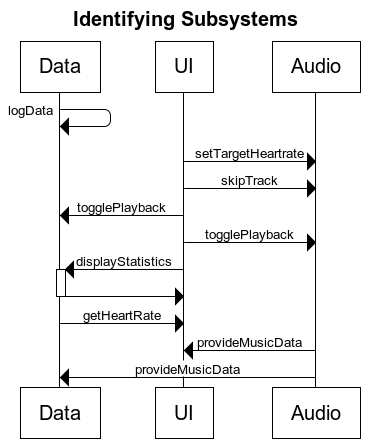
\includegraphics{img/subsystems.png}\\
        %title Identifying Subsystems
        %Data->Data:logData
        %UI->Audio:setTargetHeartrate
        %UI->Audio:skipTrack
        %UI->Data:togglePlayback
        %UI->Audio:togglePlayback
        %UI->+Data: displayStatistics
        %Data->-UI: 
        %Data->UI: getHeartRate
        %Audio->UI: provideMusicData
        %Audio->Data: provideMusicData
		\caption{Subsystems}
	\end{figure}
\end{center}

\section{Mapping Subsystems to Hardware}

\section{Persistent Data Storage}
Since Android provides full support for SQLite databases, it is the type of storage that we have chosen for the application. The wide variety of fully-developed features allows us to focus more on the actual organization and management of the data in relation to the other modules. All that is needed is a simple call to the data base to retrieve the raw data, and the custom designed objects illustrated in the Class Diagram then do their own processing on the data. SQLite allows us to store all the data specific to application on the device itself, which is advantageous for a mobile application such as ours. The goal is for the user to be able to record and view his workout data without having to use any external devices other than his phone and the chest strap, and internal data storage via the SQLite database allows our application this benefit.
	The database will be accessible only to the Data Manager and the Data Assembler. In regards to the Data Manager, the only interactions with the database will be to store the initial state of the system, store the current music track, and store the current heart rate. It will not retrieve anything from the database, because that is the purpose of the Data Assembler. The Data Assembler is the other object that will interact with the database. It will issue requests for the various data that the UI would like to graph, which include the heart rate, the current times, and the songs. Thus, the Data Manager and Data Assembler are the only objects that have direct access to the database.
\section{Network Protocol}

\section{Global Control Flow}
\subsection{Execution Orderness}
The execution order is a mix of procedure-driven and event-driven.
From a broad view, the use of the program follows the same steps: the user starts the music, the system runs, then the user stops the music.
However, the system provides a variety of interface options to activate events during the execution: a user may pause or skip playback, and view their statistics, at any time.

\subsection{Time Dependency}
The system is real-time, with a timer firing once a second.
This timer triggers the fetching of the heart rate from the monitor, and triggers the logging of this data.

\subsection{Concurrency}
The Android standard concurrency model is that the main thread handles UI, so lengthy tasks must be performed on a background thread else the UI becomes unresponsive.
As such, the network IO of the music selection system must certainly be in a different thread.
Synchronization is unnecessary as there is no shared resource.

\section{Hardware Requirements}
The system requires:
\begin{itemize}
  \item Touch screen display with minimum resolution of 640 x 480 pixels
  \item Storage space for music library, minimum size of 100 Mb
  \item Bluetooth for communication with a heart rate monitor
  \item Network connection for communicating with music selection service
  \item Audio playback capabilities
\end{itemize}
All of these requirements are met by most Android phones on the market.


\chapter{User Interface Design and Implementation}
Since we spent the time to make high quality mockups early on in this project, the UI was already well thought out and designed with standard Android UI elements such that it does not have to change much in implementation.\\
\\
One significant difference with regards to our initial design was the removal of a few features.
In the original mockup, there is a settings page with the options to change Music library location, Login, and enable music generation.
These features are nonessential, not documented in our Use Cases, and therefore will be removed from the design until essential features are delivered.
The Music library location shall be the default Android Music library location, the app shall be single-user (reasonable, since phones are personal items), and music generation is of secondary interest to music playback.\\
We also removed the About page, reasoning that the simple UI should be intuitive to the user and it would not be worth cluttering the UI with help.\\
\\
Since we now only have one element to display on the dropdown menu, we will instead have a fixed button to access the Statistics screen in place of the menu.
This halves the user effort to access the Statistics screen, now only requiring one click, therefore friendlier to the exercising user.
Otherwise, User Interface interactions remain as planned.

\chapter{Design of Tests}

\begin{center}
        \begin{tabular}{|C{15cm}|}
                \hline
                        \textbf{Increase/Decrease Target Heart Rate}\\
                \hline
                        \begin{flushleft}
                                \textbf{Test covers : } Graphical User Interface
                        \end{flushleft}
                        \begin{flushleft}
                                \textbf{Assumption: } The application is showing the correct screen.
                        \end{flushleft}
			\begin{center}
				\textbf{Integration Testing}
			\end{center}
                        \begin{flushleft}
                                \textbf{Steps:}
                        \end{flushleft}
				\begin{itemize}
					\item Press the button to increase target heart rate
					\item $\rightarrow$ If the target heart rate has diisplayed an increase in its value, press the button to decrease target heart rate
				\end{itemize}
			\begin{flushleft}
				\textbf{Expected: } Target heart rate is successfully incremented/decremented when the correct buttons are pressed
			\end{flushleft}
                        \begin{flushleft}
                                \textbf{Fails if: }
                        \end{flushleft}
                                \begin{itemize}
                                        \item Target heart rate does not change
					\item Target heart rate changes in an incorrect direction
                                \end{itemize}
				\\
		\hline
        \end{tabular}
\end{center}

\begin{center}
        \begin{tabular}{|C{15cm}|}
                \hline
                        \textbf{Start/Pause Workout (Music Playback)}\\
                \hline
                        \begin{flushleft}
                                \textbf{Test covers : } Graphical User Interface
                        \end{flushleft}
                        \begin{flushleft}
                                \textbf{Assumption: } The heart rate monitor is ready to begin collecting data and a target heart rate has been selected.
                        \end{flushleft}
			\begin{center}
				\textbf{Integration Testing}
			\end{center}
                        \begin{flushleft}
                                \textbf{Steps:}
                        \end{flushleft}
				\begin{itemize}
					\item User presses button to initialize music playback.
					\item $\rightarrow$ If the music playback successfully begins, press button to pause music playback.
				\end{itemize}
			\begin{flushleft}
				\textbf{Expected: } When the user presses the button to begin the music playback, the workout will begin. When the user presses the button pause the music playback, the music playback will pause.
			\end{flushleft}
                        \begin{flushleft}
                                \textbf{Fails if: }
                        \end{flushleft}
                                \begin{itemize}
                                        \item The music playback does not begin when the button is pressed
					\item The music playback does not pause when the button is pressed
                                \end{itemize}
				\\
		\hline
        \end{tabular}
\end{center}

\begin{center}
        \begin{tabular}{|C{15cm}|}
                \hline
                        \textbf{Skip Track}\\
                \hline
                        \begin{flushleft}
                                \textbf{Test covers : } Graphical User Interface
                        \end{flushleft}
                        \begin{flushleft}
                                \textbf{Assumption: } Application has already begun music playback and a song is currently playing.
                        \end{flushleft}
			\begin{center}
				\textbf{Integration Testing}
			\end{center}
                        \begin{flushleft}
                                \textbf{Steps:}
                        \end{flushleft}
				\begin{itemize}
					\item User presses the button to skip the current track
				\end{itemize}
			\begin{flushleft}
				\textbf{Expected: } The application will play a new song
			\end{flushleft}
                        \begin{flushleft}
                                \textbf{Fails if: }
                        \end{flushleft}
                                \begin{itemize}
					\item Pressing the button does not play the next song
                                \end{itemize}
				\\
		\hline
        \end{tabular}
\end{center}

\begin{center}
        \begin{tabular}{|C{15cm}|}
                \hline
                        \textbf{Display Graphs}\\
                \hline
                        \begin{flushleft}
                                \textbf{Test covers : } Graphical User Interface
                        \end{flushleft}
                        \begin{flushleft}
                                \textbf{Assumption: } User has logged data into the application and is on the correct screen
                        \end{flushleft}
			\begin{center}
				\textbf{Integration Testing}
			\end{center}
                        \begin{flushleft}
                                \textbf{Steps:}
                        \end{flushleft}
				\begin{itemize}
					\item User presses the button to display statistics
				\end{itemize}
			\begin{flushleft}
				\textbf{Expected: } The application will display graphs for the
			\end{flushleft} user
                        \begin{flushleft}
                                \textbf{Fails if: }
                        \end{flushleft}
                                \begin{itemize}
                                        \item The user presses the button and graphs do not display
                                \end{itemize}
				\\
		\hline
        \end{tabular}
\end{center}
\begin{center}
        \begin{tabular}{|C{15cm}|}
                \hline
                        \textbf{Music Algorithm}\\
                \hline
                        \begin{flushleft}
                                \textbf{Test covers : } Data Manager
                        \end{flushleft}
                        \begin{flushleft}
                                \textbf{Assumption: } The application has been running long enough for sufficient BPM and Heart Rate data to be logged for graphing.
                        \end{flushleft}
			\begin{center}
				\textbf{Integration Testing}
			\end{center}
                        \begin{flushleft}
                                \textbf{Steps: }
                        \end{flushleft}
				\begin{itemize}
					\item User requests a graph on Music Tempo vs Heart Rate
				\end{itemize}
			\begin{flushleft}
				\textbf{Expected: } A graph that shows Music Tempo vs Heart Rate should be displayed, and there should be an approximately linear relationship.
			\end{flushleft}
                        \begin{flushleft}
                                \textbf{Fails if: }
                        \end{flushleft}
                                \begin{itemize}
                                        \item The BPM vs Heart Rate graph does not display.
					\item The BPM vs Heart Rate graph's data does not match the expected data from the selection algorithm.
                                \end{itemize}
				\\
		\hline
        \end{tabular}
\end{center}
\begin{center}
        \begin{tabular}{|C{15cm}|}
                \hline
                        \textbf{Return from Graphs}\\
                \hline
                        \begin{flushleft}
                                \textbf{Test covers : } Graphical User Interface
                        \end{flushleft}
                        \begin{flushleft}
                                \textbf{Assumption: } The application is currently displaying graphical data.
                        \end{flushleft}
			\begin{center}
				\textbf{Integration Testing}
			\end{center}
                        \begin{flushleft}
                                \textbf{Steps:}
                        \end{flushleft}
				\begin{itemize}
					\item User presses the "back" button on the android device
				\end{itemize}
			\begin{flushleft}
				\textbf{Expected: } The application will return to the main screen from the graph display screen.
			\end{flushleft}
                        \begin{flushleft}
                                \textbf{Fails if: }
                        \end{flushleft}
                                \begin{itemize}
                                        \item The user presses the "back" button but the screen does not change.
                                \end{itemize}
				\\
		\hline
        \end{tabular}
\end{center}

Further testing must be done in order to validate the accuracy of displaying the user's current heart rate. This accuracy, however, is hard to validate because the application simply displays the number that it receives directly from the heart rate monitor. If the displayed number appears to be off, then the heart rate monitor may be faulty. Otherwise, there is no way to check whether the displayed number is the actual number that the monitor records.

\chapter{Project Management and Plan of Work}
\section{Merging Contributions}
We wrote this document in \LaTeX, so uniform formatting and appearance is guaranteed by the compiler.
We used git version control to share and merge everyone's work, such that each of us was responsible for merging elegantly when conflicts arose.
However, as half the team were beginners with both of these technologies, issues arose in improper LaTeX coding leading to compile errors.
In these cases, more experienced members would step in to fix the mistakes.

\section{Project Coordination and Progress Report}
Our project is in a unique situation where, due to teamwork disagreements, the Audio Subsystem team has split from the rest of the group.
With the professor's approval, we will be submitting two separate reports for grading.
As such, certain parts of this report pertaining to the Audio subsystem are not complete.
\\
\\
No Use Cases have yet been implemented, but for the first demo we will have a fully functional user interface and a working data logger.
Since application of the Chest Strap is a complicated process requiring the user to moisten the electrodes and strip down, for purposes of the demo the Chest Strap's output will be faked by a UI element allowing real-time modification of the reported value.
\section{Plan of Work}

\section{Breakdown of Responsibilities}
The breakdown of responsibilities follows the initial division.
\\
Revan and Tae-Min will develop the User Interface and Hardware Interface.
The Hardware Interface was a part of the User Interface in our original design, but has since been moved to the Data Logging subsystem.
As the more experienced Android developer, Revan will still be responsible for the Hardware Interface.
\\
Nikhil and Jonathan will develop the Data Logging Subsystem.
\\
Samani and Kenny will develop the Audio Subsystem, albeit independently.
\\
\\
Integration of the UI and Data subsystem will be handled by Revan and Nikhil.
\\
Since one of the elements is a UI, integration testing will be trivial and performed during integration.

\chapter*{Individual Contributions Breakdown}
\begin{center}
	\begin{tabular}{|l|C{2cm}|C{1.5cm}|C{1.5cm}|C{1.5cm}|C{1.5cm}|C{1.5cm}|}
		\hline
                        &Kenny Bambridge& Jonathan Chang& Samani Gikandi& Tae-Min Kim   & Nikhil Shenoy & Revan Sopher  \\ \hline
                        &               &               &               &               &               &               \\ \hline
%1 CSR
CSR                     &      17       &      17       &       17      &      17       &       17      &       17      \\ \hline
                        &               &               &               &               &               &               \\ \hline

%2 Sys Req
System Requirements     &               &      23       &               &               &       43      &       33      \\ \hline
Func. Requirements      &               &      50       &               &      50       &               &               \\ \hline
Non-Func. Req.          &               &               &               &               &      100      &               \\ \hline
Appearance Req.         &               &               &               &               &               &      100      \\ \hline
                        &               &               &               &               &               &               \\ \hline

%3 Func Req Spec
Stake. Actors and Goals &               &               &               &     100       &               &               \\ \hline
System Sequence Diagrams&               &               &      100      &               &               &               \\ \hline
Use Cases               &               &               &               &      36       &       43      &       20      \\ \hline
                        &               &               &               &               &               &               \\ \hline

UI Spec                 &      33       &      33       &               &               &               &       33      \\ \hline
%4 UI Spec
%reliminary Design      &               &      50       &               &               &               &       50      \\ \hline
%ser Effort Estimation  &     100       &               &               &               &               &               \\ \hline
                        &               &               &               &               &               &               \\ \hline

Domain Analysis         &      20       &               &       20      &      20       &       20      &       20      \\ \hline
%5 Domain Analysis
%omain Model            &      50       &               &       50      &               &               &               \\ \hline
%peration Contracts     &               &               &               &      50       &       50      &               \\ \hline
%athematical Model      &               &               &               &               &               &      100      \\ \hline
                        &               &               &               &               &               &               \\ \hline

%6 Plan of Work
Plan of Work            &               &     100       &               &               &               &               \\ \hline

                        &               &               &               &               &               &               \\ \hline
Total                   &      70       &     223       &      137      &     223       &      223      &      223      \\ \hline
			&		&		&		&		&		&		\\ \hline
Percentage		&	6.37\%	&	20.3\%	&	12.43\%	&	20.3\%	&	20.3\%	&	20.3\%	\\ \hline
	\end{tabular}
\end{center}

\chapter*{References}

References 1-5 are the final project reports of the previous groups who worked on the Personal Health Monitoring projects. They were consulted in conjunction with Professor Marsic's Software Engineering textbook as a guide for formatting guidelines, content ideas, and inspiration. 
\begin{verbatim}
[0] http://www.ece.rutgers.edu/~marsic/books/SE/book-SE_marsic.pdf
[1] http://www.ece.rutgers.edu/~marsic/books/SE/projects/HealthMonitor/2013-g7-report3.pdf
[2] http://www.ece.rutgers.edu/~marsic/books/SE/projects/HealthMonitor/2013-g8-report3.pdf
[3] http://www.ece.rutgers.edu/~marsic/books/SE/projects/HealthMonitor/2012-g1-report3.pdf
[4] http://www.ece.rutgers.edu/~marsic/books/SE/projects/HealthMonitor/2012-g2-report3.pdf
[5] http://www.ece.rutgers.edu/~marsic/books/SE/projects/HealthMonitor/2012-g3-report3.pdf
\end{verbatim}
Reference 6 is a review of the Motorola MOTOACTV device. They provided us with the specifications and usage details to help us develop our project proposal.
\begin{verbatim}
[7] http://reviews.cnet.com/specialized-electronics/motorola-MOTOACTV-gps-fitness/4505-3505_7-35163040.html
\end{verbatim}

References 7-8 are Wikipedia articles that helped educate us on electroencephalography and electroencephalogram define the terms for our glossary.
\begin{verbatim}
[7] http://en.wikipedia.org/wiki/Electroencephalography
[8] http://www.scholarpedia.org/article/Electroencephalogram
\end{verbatim}

Reference 9 provided us with an opening statistic to highlight the industry demand for fitness.
\begin{verbatim}
[9] http://www.statista.com/statistics/242190/us-fitness-industry-revenue-by-sector/
\end{verbatim}

References 10-11 are pictures that we used for our cover.
\begin{verbatim}
[10] https://yt4.ggpht.com/-knZVRWVniHU/AAAAAAAAAAI/AAAAAAAAAAA/QN5_n28x_R0/s900-c-k-no/photo.jpg
[11] http://www2.hu-berlin.de/fpm/graphics/logo_heartbeat-note.png
\end{verbatim}


References 12-13 are information about target heart rates.
\begin{verbatim}
[12] http://www.webmd.com/fitness-exercise/healthtool-target-heart-rate-calculator
[13] http://www.livestrong.com/article/105256-normal-heart-rate-sleeping/
\end{verbatim}

References 14-15 explain how exercise and sleep affect heart rate.
\begin{verbatim}
[14] http://www.active.com/fitness/articles/how-does-exercise-affect-your-heart
[15] http://www.webmd.com/sleep-disorders/features/how-sleep-affects-your-heart
\end{verbatim}

Reference 16 was consulted in describing the Architectural style of our system.
\begin{verbatim}
[16] http://en.wikipedia.org/wiki/Multitier_architecture
\end{verbatim}

References 17-18 were consulted in considering algorithmic design.
\begin{verbatim}
[17] http://www.urmc.rochester.edu/encyclopedia/content.aspx?ContentTypeID=1&ContentID=1209
[18] http://www.livescience.com/42081-normal-heart-rate.html
\end{verbatim}



\end{document}


%%  LocalWords:  Traceability

